%% The CEL paper. IEEE conference format (CoRL/ICRA length).
%%
%% Build:  ./build.sh          (pdflatex -> bibtex -> pdflatex x2)
%% Numbers: data/*.tex is generated by make_numbers.py from the audit's JSON
%% and CSV. Do not type a statistic into this file; if a number here disagrees
%% with the data, the build is wrong, not the prose.

\documentclass[conference]{IEEEtran}

\usepackage{amsmath,amssymb}
\usepackage{amsthm}
\usepackage{array}
\usepackage{booktabs}
\usepackage{graphicx}
\usepackage{microtype}
% The author's name is given in both scripts; CJKutf8 renders the Chinese
% characters inside the IEEEtran block without switching the document's font
% encoding or requiring a XeLaTeX build.
\usepackage{CJKutf8}
\usepackage{siunitx}
\usepackage{tikz}
\usepackage{hyperref}
\usepackage{xcolor}

\usetikzlibrary{arrows.meta,positioning,fit,backgrounds}
\sisetup{detect-all}

\theoremstyle{definition}
\newtheorem{definition}{Definition}
\newtheorem{proposition}{Proposition}

% The audit's numbers, from experiments/benchmark_libero_audit.py.
% Generated by experiments/cel_paper/make_numbers.py -- do not edit.
% Source: experiments/libero_audit_summary.json,
%         experiments/libero_audit_episodes.csv

\newcommand{\EpisodesPerArm}{100}
\newcommand{\TotalEpisodes}{200}
\newcommand{\ControlHz}{20}
\newcommand{\ChunkSteps}{6}
\newcommand{\TaskIndex}{2}
\newcommand{\MujocoVersion}{3.2.3}
\newcommand{\RobosuiteVersion}{1.4.0}
\newcommand{\GainX}{0.0115}
\newcommand{\GainY}{0.0132}
\newcommand{\GainZ}{0.0129}
\newcommand{\ModelResidual}{11.8}
\newcommand{\ModelSamples}{15}
\newcommand{\GridMm}{10}
\newcommand{\BreakerTrips}{3}
\newcommand{\LiftEpsMm}{20}
\newcommand{\PlaceToleranceMm}{50}
\newcommand{\ConfidenceGateMs}{40}
\newcommand{\MaxReplans}{6}
\newcommand{\CanonicalForm}{\texttt{scene:<plate cells>:<bowl claim>[:<bowl cells>]}}
\newcommand{\PoseDeltaMin}{101}
\newcommand{\PoseDeltaMax}{108}
\newcommand{\PoseDeltaCount}{3}
\newcommand{\SafeAll}{51.0}
\newcommand{\SafeAllLo}{41.3}
\newcommand{\SafeAllHi}{60.6}
\newcommand{\SafeAllN}{100}
\newcommand{\SafeNominal}{100.0}
\newcommand{\SafeNominalLo}{88.6}
\newcommand{\SafeNominalHi}{100.0}
\newcommand{\SafeNominalN}{30}
\newcommand{\SafePoseDrift}{0.0}
\newcommand{\SafePoseDriftLo}{0.0}
\newcommand{\SafePoseDriftHi}{7.9}
\newcommand{\SafePoseDriftN}{45}
\newcommand{\SafeChannel}{84.0}
\newcommand{\SafeChannelLo}{65.3}
\newcommand{\SafeChannelHi}{93.6}
\newcommand{\SafeChannelN}{25}
\newcommand{\CELAll}{100.0}
\newcommand{\CELAllLo}{96.3}
\newcommand{\CELAllHi}{100.0}
\newcommand{\CELAllN}{100}
\newcommand{\CELNominal}{100.0}
\newcommand{\CELNominalLo}{88.6}
\newcommand{\CELNominalHi}{100.0}
\newcommand{\CELNominalN}{30}
\newcommand{\CELPoseDrift}{100.0}
\newcommand{\CELPoseDriftLo}{92.1}
\newcommand{\CELPoseDriftHi}{100.0}
\newcommand{\CELPoseDriftN}{45}
\newcommand{\CELChannel}{100.0}
\newcommand{\CELChannelLo}{86.7}
\newcommand{\CELChannelHi}{100.0}
\newcommand{\CELChannelN}{25}
\newcommand{\PoseGap}{100.0}
\newcommand{\PoseP}{$p<10^{-24}$}
\newcommand{\AllP}{$1.3\times10^{-18}$}
\newcommand{\SafeVetoes}{84}
\newcommand{\SafeFalseVetoes}{34}
\newcommand{\SafeFalseVetoRate}{40.5}
\newcommand{\SafeFalseVetoLo}{30.6}
\newcommand{\SafeFalseVetoHi}{51.2}
\newcommand{\SafeRetries}{112}
\newcommand{\CELVetoes}{0}
\newcommand{\CELRetries}{0}
\newcommand{\CELReplans}{94}
\newcommand{\CELRefusals}{94}
\newcommand{\CELGrants}{1672}
\newcommand{\CELBreakers}{0}
\newcommand{\CELReplansPerRefusal}{1.00}
\newcommand{\CELGrantsPerEpisode}{16.7}
\newcommand{\SafeVetoesLightDim}{38}
\newcommand{\SafeFalseVetoesLightDim}{18}
\newcommand{\SafeVetoesNominal}{10}
\newcommand{\SafeFalseVetoesNominal}{5}
\newcommand{\CELRefusalsPose}{57}
\newcommand{\SafeLatency}{4609}
\newcommand{\CELLatency}{4687}
\newcommand{\CELWitnessLatency}{967}
\newcommand{\CELDecisionLatency}{3720}
\newcommand{\LatencyDelta}{78}
\newcommand{\LatencyDeltaPct}{1.7}
\newcommand{\DecisionSaving}{889}
\newcommand{\DecisionSavingPct}{19.3}
\newcommand{\CELWitnessPerChunk}{54.8}
\newcommand{\CELWitnessFirstTen}{9.9}
\newcommand{\CELWitnessLastTen}{99.8}
\newcommand{\WitnessHashUs}{0.77}
\newcommand{\SafeLatencyMedian}{4560}
\newcommand{\CELLatencyMedian}{4552}
\newcommand{\DeclaredForwardMs}{200}
\newcommand{\ChainSmallEntries}{202}
\newcommand{\ChainSmallMs}{2.2}
\newcommand{\ChainMidEntries}{1002}
\newcommand{\ChainMidMs}{10.1}
\newcommand{\ChainLargeEntries}{3002}
\newcommand{\ChainLargeMs}{31.0}
\newcommand{\ChainGrowth}{14}
\newcommand{\LedgerEntries}{3534}
\newcommand{\SafeCollisions}{68}
\newcommand{\CELCollisions}{9}
\newcommand{\SafeContactsPerEpisode}{0.68}
\newcommand{\CELContactsPerEpisode}{0.09}
\newcommand{\SafeCollisionEpisodes}{4}
\newcommand{\CELCollisionEpisodes}{4}
\newcommand{\SafeDamageEpisodes}{8}
\newcommand{\CELDamageEpisodes}{7}
\newcommand{\SafeDamageRate}{8.0}
\newcommand{\CELDamageRate}{7.0}
\newcommand{\SafeDrops}{4}
\newcommand{\CELDrops}{4}
\newcommand{\SafeChunks}{1827}
\newcommand{\CELChunks}{1766}
\newcommand{\SafeSteps}{12324}
\newcommand{\CELSteps}{11578}
\newcommand{\ConfThreshold}{0.80}
\newcommand{\SafeWorstPlateDist}{192}
\newcommand{\CELWorstPlateDist}{29}
\newcommand{\SafePosePlateDist}{113}
\newcommand{\CELPosePlateDist}{6}
\newcommand{\SafeModelError}{22.3}
\newcommand{\CELModelError}{18.4}
\newcommand{\SafeRecoveryFirst}{27}
\newcommand{\SafeRecoverySecond}{22}
\newcommand{\CELRecoveryFirst}{0}
\newcommand{\CELRecoverySecond}{0}
\newcommand{\LiftSlip}{112}
\newcommand{\LiftSlipPct}{97}
\newcommand{\LiftPayload}{112}
\newcommand{\LiftPayloadPct}{97}
\newcommand{\LiftLight}{115}
\newcommand{\LiftLightPct}{100}
\newcommand{\LiftActuator}{60}
\newcommand{\LiftActuatorPct}{53}
\newcommand{\LiftNominal}{115}
\newcommand{\FrictionSlip}{0.22}
\newcommand{\MassScale}{12}
\newcommand{\LightScale}{0.30}
\newcommand{\ActuatorScale}{0.60}
\newcommand{\ImageNominal}{118}
\newcommand{\ImageLight}{22}

% The driving audit's numbers, from experiments/ad_cel_audit.py.
% Generated by experiments/cel_paper/make_numbers.py -- do not edit.
% Source: experiments/ad_cel_summary.json,
% Source:          experiments/ad_cel_data.csv

\newcommand{\ADEpisodesPerArm}{100}
\newcommand{\ADTotalEpisodes}{200}
\newcommand{\ADWitnessHz}{10}
\newcommand{\ADReplanS}{0.50}
\newcommand{\ADPlannerHz}{2}
\newcommand{\ADHorizonS}{2.5}
\newcommand{\ADTolLat}{0.5}
\newcommand{\ADTolLon}{1.0}
\newcommand{\ADTolSpeed}{0.5}
\newcommand{\ADMuNominal}{0.90}
\newcommand{\ADMuWet}{0.35}
\newcommand{\ADTauANominal}{0.10}
\newcommand{\ADTauAWorn}{0.40}
\newcommand{\ADTauSNominal}{0.08}
\newcommand{\ADTauSWorn}{0.75}
\newcommand{\ADConfThreshold}{0.80}
\newcommand{\ADEbDecel}{6.0}
\newcommand{\ADHarshDecel}{5.0}
\newcommand{\ADLeadDecel}{8.0}
\newcommand{\ADJerkLimit}{6}
\newcommand{\ADRouteM}{280}
\newcommand{\ADLaneHalf}{1.75}
\newcommand{\ADPedNear}{30}
\newcommand{\ADPedFar}{36}
\newcommand{\ADSight}{12}
\newcommand{\ADNominalN}{34}
\newcommand{\ADNominalCollSafe}{0}
\newcommand{\ADNominalCollCEL}{0}
\newcommand{\ADNominalCollSafePct}{0.0}
\newcommand{\ADNominalCollCELPct}{0.0}
\newcommand{\ADNominalCollP}{$1.000$}
\newcommand{\ADNominalSuccSafe}{100.0}
\newcommand{\ADNominalSuccCEL}{100.0}
\newcommand{\ADNominalPaintSafe}{0}
\newcommand{\ADNominalPaintCEL}{0}
\newcommand{\ADNominalPaintP}{$1.000$}
\newcommand{\ADNominalLatSafe}{0.17}
\newcommand{\ADNominalLatCEL}{0.17}
\newcommand{\ADNominalGapSafe}{17.6}
\newcommand{\ADNominalGapCEL}{17.2}
\newcommand{\ADNominalHarshSafe}{72}
\newcommand{\ADNominalHarshCEL}{69}
\newcommand{\ADNominalEBSafe}{7}
\newcommand{\ADNominalEBEpSafe}{6}
\newcommand{\ADNominalRefCEL}{22}
\newcommand{\ADNominalRefEpCEL}{16}
\newcommand{\ADNominalTimeSafe}{32.2}
\newcommand{\ADNominalTimeCEL}{31.9}
\newcommand{\ADNominalDefSafe}{-15.7}
\newcommand{\ADNominalDefSpare}{15.7}
\newcommand{\ADNominalDefMin}{-18.2}
\newcommand{\ADNominalDefBest}{18.2}
\newcommand{\ADNominalDefMax}{-12.8}
\newcommand{\ADNominalDefN}{17}
\newcommand{\ADNominalDefCEL}{-15.7}
\newcommand{\ADWetN}{30}
\newcommand{\ADWetCollSafe}{15}
\newcommand{\ADWetCollCEL}{0}
\newcommand{\ADWetCollSafePct}{50.0}
\newcommand{\ADWetCollCELPct}{0.0}
\newcommand{\ADWetCollP}{$5.8\times10^{-6}$}
\newcommand{\ADWetSuccSafe}{50.0}
\newcommand{\ADWetSuccCEL}{100.0}
\newcommand{\ADWetPaintSafe}{0}
\newcommand{\ADWetPaintCEL}{0}
\newcommand{\ADWetPaintP}{$1.000$}
\newcommand{\ADWetLatSafe}{0.14}
\newcommand{\ADWetLatCEL}{0.12}
\newcommand{\ADWetGapSafe}{5.7}
\newcommand{\ADWetGapCEL}{11.1}
\newcommand{\ADWetHarshSafe}{94}
\newcommand{\ADWetHarshCEL}{30}
\newcommand{\ADWetEBSafe}{11}
\newcommand{\ADWetEBEpSafe}{8}
\newcommand{\ADWetRefCEL}{120}
\newcommand{\ADWetRefEpCEL}{30}
\newcommand{\ADWetTimeSafe}{31.9}
\newcommand{\ADWetTimeCEL}{33.2}
\newcommand{\ADWetDefSafe}{-0.5}
\newcommand{\ADWetDefSpare}{0.5}
\newcommand{\ADWetDefMin}{-2.2}
\newcommand{\ADWetDefBest}{2.2}
\newcommand{\ADWetDefMax}{2.7}
\newcommand{\ADWetDefN}{15}
\newcommand{\ADWetDefCEL}{-12.2}
\newcommand{\ADLagN}{26}
\newcommand{\ADLagCollSafe}{0}
\newcommand{\ADLagCollCEL}{0}
\newcommand{\ADLagCollSafePct}{0.0}
\newcommand{\ADLagCollCELPct}{0.0}
\newcommand{\ADLagCollP}{$1.000$}
\newcommand{\ADLagSuccSafe}{100.0}
\newcommand{\ADLagSuccCEL}{100.0}
\newcommand{\ADLagPaintSafe}{96}
\newcommand{\ADLagPaintCEL}{0}
\newcommand{\ADLagPaintP}{$1.1\times10^{-13}$}
\newcommand{\ADLagLatSafe}{2.75}
\newcommand{\ADLagLatCEL}{0.67}
\newcommand{\ADLagGapSafe}{17.3}
\newcommand{\ADLagGapCEL}{19.5}
\newcommand{\ADLagHarshSafe}{59}
\newcommand{\ADLagHarshCEL}{64}
\newcommand{\ADLagEBSafe}{9}
\newcommand{\ADLagEBEpSafe}{7}
\newcommand{\ADLagRefCEL}{11}
\newcommand{\ADLagRefEpCEL}{10}
\newcommand{\ADLagTimeSafe}{32.8}
\newcommand{\ADLagTimeCEL}{32.3}
\newcommand{\ADLagDefSafe}{-11.0}
\newcommand{\ADLagDefSpare}{11.0}
\newcommand{\ADLagDefMin}{-19.5}
\newcommand{\ADLagDefBest}{19.5}
\newcommand{\ADLagDefMax}{-8.2}
\newcommand{\ADLagDefN}{13}
\newcommand{\ADLagDefCEL}{-10.1}
\newcommand{\ADWetLagN}{10}
\newcommand{\ADWetLagCollSafe}{5}
\newcommand{\ADWetLagCollCEL}{0}
\newcommand{\ADWetLagCollSafePct}{50.0}
\newcommand{\ADWetLagCollCELPct}{0.0}
\newcommand{\ADWetLagCollP}{$0.033$}
\newcommand{\ADWetLagSuccSafe}{50.0}
\newcommand{\ADWetLagSuccCEL}{100.0}
\newcommand{\ADWetLagPaintSafe}{10}
\newcommand{\ADWetLagPaintCEL}{0}
\newcommand{\ADWetLagPaintP}{$1.000$}
\newcommand{\ADWetLagLatSafe}{1.48}
\newcommand{\ADWetLagLatCEL}{0.41}
\newcommand{\ADWetLagGapSafe}{3.6}
\newcommand{\ADWetLagGapCEL}{13.9}
\newcommand{\ADWetLagHarshSafe}{31}
\newcommand{\ADWetLagHarshCEL}{14}
\newcommand{\ADWetLagEBSafe}{1}
\newcommand{\ADWetLagEBEpSafe}{1}
\newcommand{\ADWetLagRefCEL}{42}
\newcommand{\ADWetLagRefEpCEL}{10}
\newcommand{\ADWetLagTimeSafe}{32.6}
\newcommand{\ADWetLagTimeCEL}{33.5}
\newcommand{\ADWetLagDefSafe}{5.0}
\newcommand{\ADWetLagDefSpare}{5.0}
\newcommand{\ADWetLagDefMin}{1.6}
\newcommand{\ADWetLagDefBest}{1.6}
\newcommand{\ADWetLagDefMax}{7.3}
\newcommand{\ADWetLagDefN}{4}
\newcommand{\ADWetLagDefCEL}{-8.0}
\newcommand{\ADSafeSucc}{80.0}
\newcommand{\ADCELSucc}{100.0}
\newcommand{\ADSafeSuccLo}{71.1}
\newcommand{\ADCELSuccLo}{96.3}
\newcommand{\ADSafeSuccHi}{86.7}
\newcommand{\ADCELSuccHi}{100.0}
\newcommand{\ADSafeCollN}{20}
\newcommand{\ADCELCollN}{0}
\newcommand{\ADSafeCollPct}{20.0}
\newcommand{\ADCELCollPct}{0.0}
\newcommand{\ADCollP}{$6.6\times10^{-7}$}
\newcommand{\ADSuccP}{$6.6\times10^{-7}$}
\newcommand{\ADSafeHarsh}{256}
\newcommand{\ADCELHarsh}{177}
\newcommand{\ADSafeEBN}{28}
\newcommand{\ADSafeEBFalseEp}{19}
\newcommand{\ADSafeEBFalsePct}{19}
\newcommand{\ADCELRef}{195}
\newcommand{\ADCELRefEp}{46}
\newcommand{\ADCELRefEpPct}{46}
\newcommand{\ADCELWitnessChecks}{32586}
\newcommand{\ADCELReplans}{6665}
\newcommand{\ADTimeArrSafe}{32.4}
\newcommand{\ADTimeArrCEL}{32.6}
\newcommand{\ADTimeArrDelta}{0.2}
\newcommand{\ADTimeArrPct}{0.6}
\newcommand{\ADTimeEpSafe}{30.7}
\newcommand{\ADTimeEpCEL}{32.6}
\newcommand{\ADTimeEpDelta}{1.9}
\newcommand{\ADTimeEpPct}{6.1}
\newcommand{\ADTimeEarlySafe}{1.7}
\newcommand{\ADNominalTimeDelta}{0.3}
\newcommand{\ADMuWetG}{3.4}
\newcommand{\ADRegistrations}{39990}
\newcommand{\ADGrants}{32391}
\newcommand{\ADLedgerRefusals}{195}
\newcommand{\ADReplays}{0}
\newcommand{\ADWetImpact}{7.2}
\newcommand{\ADWetPedN}{15}
\newcommand{\ADWetPedNoEB}{12}
\newcommand{\ADWetPedEB}{3}
\newcommand{\ADWetPedSpeed}{13.8}
\newcommand{\ADTrackLag}{0.20}
\newcommand{\ADWetLatDist}{2.8}
\newcommand{\ADMuHat}{0.350}
\newcommand{\ADTauAHat}{0.400}
\newcommand{\ADTauSHat}{0.742}
\newcommand{\ADTauSHatLo}{0.722}
\newcommand{\ADTauSHatHi}{0.843}
\newcommand{\ADMuNominalHat}{0.900}
\newcommand{\ADTraceEp}{35}
\newcommand{\ADTracePedT}{21.0}
\newcommand{\ADTraceVGate}{13.8}
\newcommand{\ADTraceVCEL}{10.6}
\newcommand{\ADTraceGateBrakeDelay}{0.85}
\newcommand{\ADTraceImpact}{7.3}
\newcommand{\ADTraceCELStopT}{4.7}
\newcommand{\ADTraceCELBrakeDelay}{1.45}


\newcommand{\lib}{\texttt{libero\_spatial}}
\newcommand{\code}[1]{\texttt{#1}}

\hypersetup{
  pdftitle={Catching Physical Hallucinations: A Causal Execution Layer for VLA and Autonomous Driving under Distribution Shift},
  pdfauthor={Zhizhi Liao (\texorpdfstring{\begin{CJK}{UTF8}{gbsn}廖至智\end{CJK}}{Liao Zhizhi})},
  pdfkeywords={vision-language-action, runtime verification, causal interface, robot manipulation, autonomous driving, distribution shift}
}

\begin{document}

\title{Catching Physical Hallucinations: A Causal Execution Layer for\\
VLA and Autonomous Driving under Distribution Shift}

\author{%
\IEEEauthorblockN{Zhizhi Liao (\begin{CJK}{UTF8}{gbsn}廖至智\end{CJK})}
\IEEEauthorblockA{Independent Researcher\\
Email: \texttt{liaozhizhi@foxmail.com}}
}

\maketitle

\begin{abstract}
Vision-language-action (VLA) policies are trained to produce actions, not to
know when their actions stopped being true. Their one self-assessment is a
scalar confidence, and a confidence is a function of the model while physical
drift is a function of the world; the two can disagree without either being
wrong. We describe a \emph{causal execution layer} (CEL)---in one phrase, a
\emph{causal auditor} of the policy's own physical claims---that replaces the
question ``how sure am I?'' with ``did the world do what I said it would?''. It
never filters, clips or blocks an action: it audits the claim attached to one.
Before each action chunk the layer registers the physical consequence its world
model predicts; after the chunk it measures the consequence, quantises it in the
plan's own frame, and offers it to a hash-linked gateway. A matching digest earns
an \emph{execution warranty}---evidence, bound to this attempt, that the
commitment was redeemed. A refusal is written to the ledger and the plan is
\emph{re-derived} from the observed state rather than retried. On \lib{} task~2
(200 episodes, two arms, identical policy) the layer raises success from
\SafeAll\%\ to \CELAll\%; under a \PoseDeltaMin--\PoseDeltaMax\,mm displacement of the target plate it is
\CELPoseDrift\%\ against \SafePoseDrift\%\ ($p<10^{-24}$); and the confidence
baseline refuses \SafeFalseVetoes\ of \SafeVetoes\ actions that would have
succeeded. Total latency rises \LatencyDeltaPct\%\ while decision latency falls
\DecisionSavingPct\%, because the layer never pays for a blind retry.

The layer is not specific to an arm. We move it to an autonomous-driving stack,
where the drifted quantity is the friction of the road rather than the pose of
an object and no camera observes it: on \ADEpisodesPerArm{} episodes of a
\SI{\ADRouteM}{m} urban route, a confidence-gated planner ends \ADWetCollSafe{}
of \ADWetN{} wet-road episodes in a pedestrian collision and the layer ends
none (Fisher \ADWetCollP); in a worn-steering channel where both arms reach the
goal every time, \ADLagPaintSafe\%\ of the baseline's episodes arrive over the
centre line against \ADLagPaintCEL\%. The same layer also recovers the physical
parameters it was never given, $\hat\mu=\ADMuHat$ and
$\hat\tau_a=\ADTauAHat$\,s, from its own saturated and stepped responses.

We also report a defect in our own first implementation: the gate was a
set-membership
test over all previously registered digests, so a scene that \emph{regressed}
to an earlier state was accepted as evidence that the action had worked. Three
episodes passed every witness check with the manipulated object 245--269\,mm
from its target. A hash binds content; causation is a relation between a
prediction and a particular attempt. Binding a monotonic ordinal into every
registration closes the replay, and we argue this is a general requirement for
any physical witness, not a bug fix.
\end{abstract}

\begin{IEEEkeywords}
vision-language-action models, runtime verification, physical grounding,
causal interfaces, robot manipulation, distribution shift
\end{IEEEkeywords}

\section{Introduction}

The dominant interface between a language-level instruction and a torque-level
action is now a single learned function: a vision-language-action model maps an
image and a token sequence to a short action chunk \cite{brohan2023rt2,
kim2024openvla, black2024pi0}. Its evaluation, by construction, is nominal.
LIBERO \cite{liu2023libero} and its harnesses measure success on the
distribution the policy was trained on; when the distribution moves---a bumped
table, a worn motor, a dimmed lamp---the policy does not notice, because
nothing in it is a measurement of the world. It is a measurement of images.

The industry's answer is a confidence gate: act only if the policy reports a
sufficient scalar, otherwise refuse or hand over
\cite{alshiekh2018shielding, zhang2025safevla}. A more principled version of the
same move is a safety filter or a control barrier function, which certifies the
proposed input against a model of the dynamics
\cite{wabersich2021safetyfilter, ames2019cbf}; the newest VLA instantiation
adds such a layer to a manipulation policy and reports large safety gains on a
LIBERO variant \cite{hu2025vlsa}. These are real mechanisms, and they are the
right baselines, but they share one assumption and therefore one blind spot.
A confidence is $f(\text{model})$. Drift is $g(\text{world})$. When the world
moves and the input distribution does not, $f$ is entitled to be high and wrong.
Conversely, when the input distribution moves but the physics has not---a dimmer
light, a shadow---$f$ is entitled to be low and right. The two failure modes are
not opposite ends of one dial; they are different functions. A safety filter
narrows the same gap without closing it: it is exact with respect to the model
it is given, so a model that is wrong about the road is enforced faithfully.

This paper asks what changes if the gate is a \emph{measurement of the
consequence} instead of an opinion about the action. The layer is small. Before
a chunk runs, its world model predicts the physical state at the end of that
chunk and registers the prediction, canonicalised and hashed, with a
hash-linked gateway. After the chunk, the \emph{actual} physical state is read,
canonicalised the same way, and offered as a witness. The gateway issues an
execution warranty only for a digest that was registered before the request
arrived. If it
refuses, the ledger records the refusal and the layer re-plans from the
observation, resuming at the stage the world is actually in. The layer is
therefore an auditor of physical truth and not a filter on action: it holds no
safe set, states no constraint, and has no authority to clip a command---it
decides only whether the claim that justified the command was true. The claim is
narrow and falsifiable: \emph{a witness that commits to a physical consequence
distinguishes drift from uncertainty in a way a confidence cannot.}

\paragraph{Contributions}
\begin{enumerate}
\item A causal execution layer for chunked VLA rollouts, with the witness
defined in the plan's own reference frame so that grid quantisation does not
manufacture refusals at cell boundaries
(Section~\ref{sec:layer}).
\item A controlled comparison on a real simulator: 200 episodes of \lib{} task
2, two arms sharing one policy byte-for-byte, so the only difference is the
gate. Success \SafeAll\%\ vs \CELAll\%; under pose drift
\SafePoseDrift\%\ vs \CELPoseDrift\%; \SafeFalseVetoes\ false vetoes against
zero (Section~\ref{sec:results}).
\item A latency decomposition that separates \emph{decision} latency from
\emph{tamper-evidence} latency, and the negative result that our own chain
verification is $O(\text{ledger})$: total latency is
$+\LatencyDelta$\,ms ($+\LatencyDeltaPct\%$) while decision latency is
$-\DecisionSaving$\,ms ($-\DecisionSavingPct\%$) (Section~\ref{sec:latency}).
\item A transfer of the same layer to autonomous driving, where the drifted
quantity is a coefficient of friction instead of a pose and the outcome is a
collision instead of a completed task: \ADWetCollSafe{} collisions in
\ADWetN{} wet-road episodes against zero (Fisher \ADWetCollP), and a
worn-steering channel in which \ADLagPaintSafe\%\ of the baseline's successful
episodes arrive over the centre line against none
(Section~\ref{sec:driving}).
\item A defect in the layer itself, reported rather than patched: the first
version of the gate accepted a scene that had \emph{regressed} to a state it
had legitimately predicted earlier, because the gateway's registration set is
not consumed. A hash binds content, not causation. The fix---a one-shot
monotonic ordinal bound into every registration---is a general requirement for
physical witnesses, and the reasoning is the strongest evidence we have for the
paper's own thesis (Section~\ref{sec:err004}).
\end{enumerate}

The last item is deliberately in the abstract. A paper arguing that unbound
witnesses are worthless should not be believed on the strength of its own
witness without saying where that witness failed.

\section{Related Work}

\paragraph{VLA policies.} RT-2 \cite{brohan2023rt2}, OpenVLA
\cite{kim2024openvla} and $\pi_0$ \cite{black2024pi0} established the
image-to-action-chunk interface this paper takes as given. None of them carries
a runtime check: the policy is a function, and safety is expected to come from
the data or from a downstream filter. We take the interface as fixed and add
the check.

\paragraph{Shielding, safety filters and control barrier functions.} Shielding
\cite{alshiekh2018shielding} restricts an agent to a set of safe actions using a
model of the environment; runtime verification \cite{bartocci2018runtime,%
katz2017reluplex} checks a trace against a specification. The control-theoretic
relatives are the predictive safety filter \cite{wabersich2021safetyfilter},
which admits or minimally modifies a proposed input against a backup trajectory
computed from a learned model, and the control barrier function
\cite{ames2019cbf}, which enforces invariance of a safe set as a constraint on
the input. These are the strongest mechanisms in the literature and the closest
to ours in placement: they too sit between a policy and an actuator.

The difference is what they assume and what they measure. A CBF certifies
safety \emph{given} a safe set and a model of the dynamics; a predictive safety
filter does the same given a model and its uncertainty bound. Stating such a
specification at deployment is one of the concrete problems in safety identified
a decade ago \cite{amodei2016concrete}, and it is why both guarantees inherit
the model the designer supplies. They are correct when the model is right, and
the drift this paper is about is the case where it is not: a friction
coefficient that changed, a steering rack that lags. The guarantee then degrades
silently, because the quantity that moved is inside the model rather than in the
observation. Our witness does not certify safety at all; it makes the model's
error \emph{observable} by comparing a registered prediction with a measured
consequence, and then re-estimates from the consequence. CEL is not a shield, a
safety layer or a safety filter: it has no safe set, certifies nothing, and never
touches the action---it is a causal auditor of physical claims whose only outputs
are an execution warranty and, when the claim is false, a refusal to issue one. A
safety filter asks
``is this action safe under my model?''; we ask ``was my model true about this
action?'', which is answerable when the first is not.

\paragraph{Runtime guardrails for VLA.} The 2025 wave of VLA safety work is the
nearest neighbour and deserves to be named. SafeVLA
\cite{zhang2025safevla} folds safety into training as a constrained MDP;
VLSA/AEGIS \cite{hu2025vlsa} adds a plug-and-play control-barrier layer that
monitors a VLA's action in real time and intervenes only on predicted
violations; RoboSafe \cite{wang2025robosafe} runs a guardrail model that emits
executable safety predicates and re-plans when they are violated; AnySafe
\cite{agrawal2025anysafe} synthesises latent safety filters inside a world model
and calibrates the threshold conformally. All four are runtime interventions
between the policy and the plant, and VLSA/AEGIS is evaluated on a LIBERO
variant, which makes the comparison concrete rather than philosophical.

Two things separate this paper. First, each mechanism requires a constraint to
be \emph{stated}---an obstacle geometry, a set of unsafe predicates, a latent
failure set---whereas CEL's specification is the policy's own next-state
prediction, regenerated every chunk. Second, they modify or block the action to
keep the system inside a set; we leave the action untouched, accept or refuse
the \emph{claim}, and re-derive the plan from the measured state. A guardrail
that stops the robot when it is unsure is a veto; a witness that says ``the bowl
is on the table, so the transport stage is fiction'' is a re-estimate, and
Section~\ref{sec:results} prices the difference in false vetoes. Nothing here
diminishes the guardrail line: it is stronger than ours wherever a constraint
can be written down, and weaker exactly where the world has moved and the
constraint has not.

\paragraph{Uncertainty gating.} SafeVLA \cite{zhang2025safevla} aligns a VLA
with safety constraints in training; the classic inference-time version is a
confidence threshold. We implement the inference-time version as arm~A at its
published threshold and price its refusals counterfactually, because a refusal
rate alone cannot distinguish caution from blindness. The distribution-shift
literature reaches the same conclusion from the other side: conformal guarantees
computed on the training environment collapse when deployment differs, and the
repairs either re-estimate the shift online \cite{rahaman2026environments} or
model the uncertainty inside the planner. Both make a scalar carry information
about the world; a witness replaces the scalar with a measurement.

\paragraph{Causal framing.} DoWhy \cite{sharma2020dowhy} formalises the
do-operator for observational data. Our witness is a do-test executed on a
simulator: we do not infer $P(s'\mid \mathrm{do}(a))$, we measure it, once per
chunk, and compare it with the model's prediction. The comparison is the causal
claim. The closest work in this direction is CADET \cite{guo2026cadet}, which
audits a deployed end-to-end driving planner for reliance on cues that cannot
physically influence the decision, and repairs it by masking those queries at
test time. CADET audits the \emph{input} dependence of a plan with an offline
physics-geometric prior; we audit the \emph{outcome} of an executed plan against
a prediction registered before it ran. An input audit cannot see a drift that
leaves the input distribution intact---a wet road looks like a dry one---and an
outcome audit can, which is the experiment of Section~\ref{sec:driving}.

\paragraph{World models and physical hallucination.} Learned world models
\cite{ha2018worldmodels} are now the substrate for robot data generation, and
their characteristic failure has a name: physical hallucination, in which
generated rollouts interpenetrate objects or violate kinematics
\cite{zhou2026groundeddreamer}. The remedy is verification against a simulator
or a geometric prior \cite{zhou2026groundeddreamer, lu2026causalplan}, which is
available offline and not at execution time on a physical robot, where the only
oracle left is the plant itself.

\paragraph{End-to-end driving.} UniAD \cite{hu2023uniad} makes planning the
objective of one network over a learned scene representation and VAD
\cite{chen2023vad} vectorises the scene and samples trajectories from it; both
are scored on completing a route without contact, on the distribution they were
trained on. The output is a trajectory and a confidence, so the interface is
unchanged---and the quantity that separates a safe plan from a fatal one, the
friction of the surface, is not in the input. Section~\ref{sec:driving} runs
the comparison there.

\section{The Layer}
\label{sec:layer}

Fig.~\ref{fig:arch} fixes the vocabulary for the rest of the paper: a plan, a
commitment registered before it is executed, a measurement after, and a gateway
that either issues the warranty or refuses. Everything in this section is one of
those four boxes.

\subsection{Commitments, not opinions}

A rollout is a sequence of chunks. At chunk $k$ the policy observes $s_k$ and
emits an action chunk $a_k$ (\ChunkSteps{} control steps, \SI{0.3}{s}) together
with the physical state it expects to see afterwards.
The expectation is the model's, not ours; in our implementation it is a
per-axis gain fitted once on nominal episodes
($\GainX$, $\GainY$, $\GainZ$\,m per unit command per step, residual
$\ModelResidual$\,mm over $\ModelSamples$ probes) and frozen before any drift is
applied.

\begin{definition}[Commitment]
For chunk $k$ with observation $s_k$ and action $a_k$, the commitment is the
pair $C_k = \langle \hat{s}_{k+1},\, k\rangle$ where
$\hat{s}_{k+1} = f(s_k, a_k)$ is the model's predicted physical state after
$a_k$. The commitment is \emph{registered} before $a_k$ is executed.
\end{definition}

The registration is what makes the check causal rather than post-hoc. A
prediction written after the fact can always be fitted to what happened; a
prediction written before, hashed, and appended to an append-only chain cannot.

The artifact a match returns is the \emph{execution warranty}: a statement,
verifiable later, that the commitment of one particular attempt was redeemed by
the plant. It is a receipt for a claim, not a permission to act---the action in
Arm~B is the policy's, unmodified. This is the sense in which the layer audits
rather than filters: an unmodified action with a checkable warranty is an audit
trail, whereas a clipped action has lost the evidence of what the policy
wanted.

\subsection{The witness}

The observed state is reduced to the part the plan can assert something about:
the target object's pose and a three-valued classification of the manipulated
object,
\[
\text{bowl} \in \{\textsf{table},\ \textsf{gripped},\ \textsf{placed}\},
\]
decided from geometry with a declared \LiftEpsMm\,mm lift threshold (a successful
grasp lifts the bowl \SI{85}{mm}; a missed one lifts nothing) and a declared
\PlaceToleranceMm\,mm placement tolerance. The end effector is deliberately \emph{absent} from
the witness: the controller measures it every step, so including it would let
the witness be right for the wrong reason.

\paragraph{Quantise the displacement, not the coordinate.}
A digest over raw coordinates is unstable at cell boundaries: an object that
happens to sit on a grid line flips its hash under sub-millimetre jitter, and
the gate refuses for a reason that has nothing to do with the world. We
therefore canonicalise in the plan's frame,
\begin{equation}
\kappa(s) = \Bigl\lfloor \tfrac{s_{\text{plate}} - b_{\text{plate}}}{g}
\Bigr\rceil \;\Vert\; \text{claim}(s),
\qquad g = \GridMm\,\text{mm},
\end{equation}
where $b$ is the plan's belief. Both sides quantise the same reference, so only
the \emph{displacement} is exposed to the grid. Ten millimetres is measured, not
tuned: the plate and a resting bowl are predicted to sub-millimetre accuracy,
but the plate itself settles by about \SI{1}{mm} when a bowl is set down on it,
and the smallest drift we inject is \SI{80}{mm}. A \SI{10}{mm} grid is five
times the settling and an eighth of the signal.

\subsection{Refusal is a re-estimate, not a retry}

When the gateway refuses, the layer does not replay the chunk. It treats the
pair $(\hat{s}_{k+1}, s_{k+1})$ as a measurement and asks a different question:
\emph{what stage is the world in?} The plan's grasp and placement targets are
re-derived from the fresh observation, the per-axis gain is re-fitted from the
prediction error, and the program resumes at the stage implied by the observed
classification:

\begin{center}
\small
\begin{tabular}{ll}
\toprule
Observed & Resume at \\
\midrule
\textsf{gripped} & wherever the plan was, if it was carrying \\
\textsf{table} & \textsf{approach}, i.e.\ grasp again \\
\textsf{placed} & \textsf{retreat}, i.e.\ let go and back off \\
\bottomrule
\end{tabular}
\end{center}

This is the substantive difference from a confidence gate. A retry says ``try
the same thing again''; a re-derivation says ``the bowl is on the table, so the
transport stage is fiction, start from the pick''. In our run the layer pays
$\CELReplans$ re-derivations over $\EpisodesPerArm$ episodes, exactly one per
refusal, and none of them is a repeat of a failed action.

\subsection{The breaker}

\BreakerTrips{} consecutive refusals, or \MaxReplans{} re-derivations in one episode, trip a
circuit breaker and the episode is abandoned with a recorded reason. The
breaker is not a safety mechanism; it is a \emph{price} on the absence of
progress. A plan that keeps paying forward passes for a world it cannot satisfy
is the failure the layer exists to make visible.

\begin{figure*}[t]
\centering
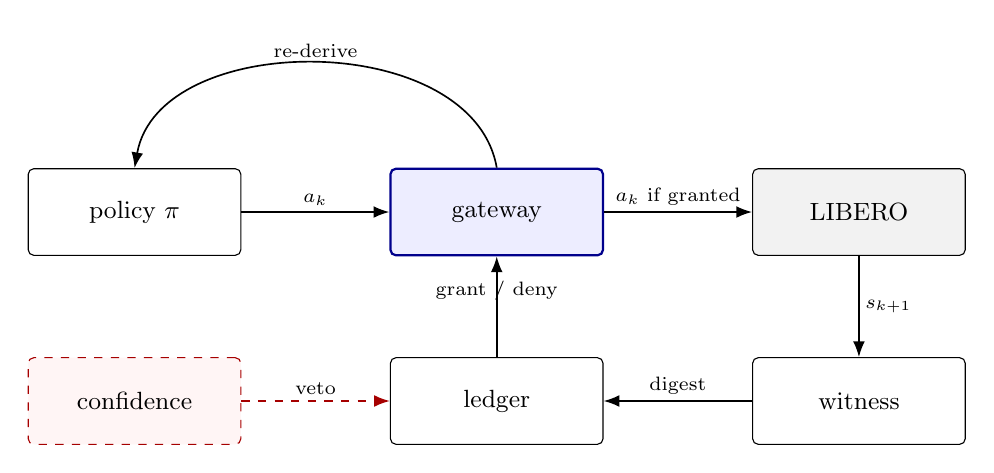
\begin{tikzpicture}[
  font=\small,
  x=1cm, y=1cm,
  box/.style={draw, rounded corners=2pt, align=center, inner sep=4pt,
              minimum width=27mm, minimum height=11mm},
  gate/.style={box, fill=blue!7, draw=blue!55!black, thick},
  phys/.style={box, fill=black!5},
  arm/.style={-{Latex[length=2mm]}, semithick},
  mis/.style={-{Latex[length=2mm]}, semithick, dashed, draw=red!65!black},
  lbl/.style={font=\scriptsize, inner sep=2pt},
]
\node[box]  (pol)  at (0.0,0.0)   {policy $\pi$};
\node[gate] (gate) at (4.6,0.0)   {gateway};
\node[phys] (env)  at (9.2,0.0)   {LIBERO};
\node[box]  (wit)  at (9.2,-2.4)  {witness};
\node[box]  (led)  at (4.6,-2.4)  {ledger};
\node[box, dashed, draw=red!65!black, fill=red!4] (conf) at (0.0,-2.4)
  {confidence};

\draw[arm] (pol)  -- node[lbl, above]{$a_k$} (gate);
\draw[arm] (gate) -- node[lbl, above]{$a_k$ if granted} (env);
\draw[arm] (env)  -- node[lbl, right]{$s_{k+1}$} (wit);
\draw[arm] (wit)  -- node[lbl, above]{digest} (led);
\draw[arm] (led)  -- node[lbl, above]{grant / deny} (gate);
\draw[arm] (gate.north) to[out=100,in=80] node[lbl, above]{re-derive} (pol.north);
\draw[mis] (conf) -- node[lbl, above]{veto} (led);
\end{tikzpicture}
\caption{The layer. Arm~B routes every action chunk $a_k$ through a gateway that
issues an execution warranty only for a physical consequence registered \emph{before} the
chunk ran; the state $s_{k+1}$ is read after the chunk, canonicalised by the
witness, and offered to the ledger. A refusal re-derives the plan from
$s_{k+1}$. Arm~A (dashed) replaces the witness with a threshold on the policy's
own confidence, so its only input is the model. Both arms drive the same
simulator with the same action interface; the gate is the entire difference.}
\label{fig:arch}
\end{figure*}

\section{Experimental Protocol}
\label{sec:protocol}

\paragraph{Environment.} \lib{} task \TaskIndex{}---``pick up the black bowl
from table center and place it on the plate''---through
\code{OffScreenRenderEnv} on MuJoCo \MujocoVersion{} \cite{todorov2012mujoco}
(pinned, not relaxed for this experiment) and robosuite \RobosuiteVersion{}
\cite{zhu2020robosuite}, rendering under
EGL. Actions are the standard 7-DoF OSC delta pose at \ControlHz\,Hz; a chunk
is \ChunkSteps{} steps, \SI{0.3}{s} of committed motion. This is the interface
every LIBERO policy emits, not a bespoke one.

\paragraph{One policy, two gates.} Both arms share a single chunked
pick-and-place program: plan targets once from the first observation, commit to
six-step chunks, servo within a chunk from proprioception. The policy is
open-loop \emph{within} a chunk on purpose---that is what a VLA is---so the
comparison cannot be explained by feedback control that re-reads the world at
every step.
The arms differ only in what sits between the policy and the actuator.

\paragraph{Arm A (confidence-gated baseline).} Veto any chunk whose confidence is below
\ConfThreshold, retry up to three times, then execute anyway: a VLA cannot skip
its own action chunk, so a gate without an abandon path converts uncertainty
into latency rather than into safety. The confidence signal is the model of a
policy head described in Section~\ref{sec:threats}; its input is the mean
brightness of the delivered frame, because that is the quantity a confidence
head actually degrades with.

\paragraph{Arm B (CEL).} As in Section~\ref{sec:layer}, with a
\code{MembraneGateway} issuing execution warranties against pre-registered digests and
writing every grant and denial to a hash-linked ledger.

\paragraph{False vetoes are priced, not assumed.} A veto is counted as false
only if replaying the vetoed chunk on a snapshot of the simulator advances the
task or brings the bowl measurably closer to the plate. The replay is
bookkeeping: it restores the snapshot and the episode's step, contact and drop
counters, so the counterfactual never contaminates the run it scores.

\paragraph{Drift.} Five channels, all applied to the MuJoCo model and never to
the observation: \emph{pose drift} (the plate is displaced at the transport
boundary), \emph{surface slip} (all sliding frictions to $\FrictionSlip$),
\emph{payload} (bowl mass $\times\MassScale$), \emph{light} (headlight to $\LightScale$), and
\emph{actuator} (\code{actuator\_gainprm} to $\ActuatorScale$). The schedule is an
explicit list, identical for both arms: \SafeNominalN{} nominal episodes,
$\SafePoseDriftN$ under pose drift in two blocks, then the four physical
channels. Table~\ref{tab:regime} splits the results the same way.

\paragraph{The drift displacements are measured, not chosen.} This matters more
than it looks. Two constraints pin the three pose-drift vectors. First, the
arm's steady-state error grows to \SIrange{10}{100}{mm} beyond
$x\approx\SI{0.03}{m}$, $y\approx\SI{0.30}{m}$, so a plate bumped there is
outside the precise workspace and \emph{no} planner can place on it; an
experiment that bumps it there measures the arm's reach, not the layer.
Second, the plate must stay clear of the neighbouring bowl at
$(0.009, 0.306)$\,m: a displacement that parks the plate inside that footprint
leaves a gap too narrow for a \SI{94}{mm} bowl, and LIBERO's \code{on}
predicate---which requires actual contact---becomes unsatisfiable for any
policy. All \PoseDeltaCount{} vectors move the plate \PoseDeltaMin--\PoseDeltaMax\,mm through
the region the arm tracks to sub-\SI{2}{mm}. We found both failure modes by
running them; they are recorded because a benchmark that silently contains
unsatisfiable episodes is not measuring the interface.

\paragraph{The latency ledger is arithmetic, and can be re-priced.} Two costs
are declared rather than measured---one forward pass
$c_f=\DeclaredForwardMs$\,ms, one confidence gate $c_g=\ConfidenceGateMs$\,ms---and everything else
is measured. With $N$ chunks, $R$ retries, $P$ re-derivations, $W$ witness time
and $E$ episodes,
\begin{equation}
\begin{aligned}
L_A &= \frac{N_A(c_f + c_g) + R_A c_f}{E},\\
L_B &= \frac{(N_B + P_B)\,c_f}{E} + W_B .
\end{aligned}
\label{eq:latency}
\end{equation}
Substituting $N_A=\SafeChunks$, $R_A=\SafeRetries$, $N_B=\CELChunks$,
$P_B=\CELReplans$, $W_B=\CELWitnessLatency$\,ms/\mbox{episode} reproduces the
reported means to the millisecond, which means a reader who disagrees with
$c_f$ can re-price both arms without re-running anything.

\paragraph{Statistics.} Proportions carry 95\,\% Wilson intervals, which unlike
the normal approximation stay inside $[0,1]$ at the four cells that are $0$ or
$n$. The two arm-level comparisons are Fisher exact tests, for the same reason.

% Generated by make_numbers.py -- do not edit.
\begin{table*}[t]
\centering
\caption{The two arms on \texttt{libero\_spatial} task 2, 100 episodes each. Brackets are 95\,\% Wilson intervals (not reported by the harness; computed by \texttt{make\_numbers.py}). Latency is per completed episode and includes the arm's own retries; the decomposition in Table~\ref{tab:witnesscost} is the one to read.}
\label{tab:main}
\begin{tabular}{lrrl}
\toprule
 & \textbf{Conf.-gated} & \textbf{CEL} & \textbf{Diff. (pts)} \\
\midrule
\multicolumn{4}{l}{\emph{Success}} \\
Success, all episodes (n=100) & 51.0\,[41.3--60.6] & 100.0\,[96.3--100.0] & $+49.0$ \\
Success, nominal (n=30) & 100.0\,[88.6--100.0] & 100.0\,[88.6--100.0] & $0$ \\
Success, pose drift (n=45) & 0.0\,[0.0--7.9] & 100.0\,[92.1--100.0] & $+100.0$ \\
Success, physical channels (n=25) & 84.0\,[65.3--93.6] & 100.0\,[86.7--100.0] & $+16.0$ \\
\addlinespace
\multicolumn{4}{l}{\emph{What the gate did}} \\
Vetoes / retries & 84 / 112 & 0 / 0 & \\
Re-derivations from a witness & $0$ & 94 & \\
False vetoes / refusals & 34/84 = 40.5\% & $0$ & \\
Episodes to recover after onset & 27, 22 & 0, 0 & \\
\addlinespace
\multicolumn{4}{l}{\emph{Physical cost}} \\
Contacts (total / per episode) & 68 / 0.68 & 9 / 0.09 & \\
Episodes with damage & 8 / 100 & 7 / 100 & \\
Worst final bowl--plate gap & 192 mm & 29 mm & \\
\addlinespace
\multicolumn{4}{l}{\emph{Latency per episode}} \\
Total policy latency & 4609 ms & 4687 ms & \\
\quad of which tamper-evidence & $0$ ms & 967 ms & \\
\quad of which decision & 4609 ms & 3720 ms & \\
\bottomrule
\end{tabular}
\end{table*}


% Generated by make_numbers.py -- do not edit.
\begin{table}[!htbp]
\centering
\footnotesize
\setlength{\tabcolsep}{4pt}
\caption{The same 100 episodes, split by the world they ran in. \emph{False} counts vetoes that the counterfactual replay shows would have advanced the task; \emph{ref.} counts CEL's witness refusals, every one of which the ledger records as a measured mismatch.}
\label{tab:regime}
\begin{tabular}{lrrrrr}
\toprule
World & $n$ & \multicolumn{2}{c}{Success} & \multicolumn{2}{c}{Gate} \\
\cmidrule(lr){3-4}\cmidrule(lr){5-6}
 & & Safe & CEL & veto (false) & refusals \\
\midrule
nominal & 30 & 100.0 & 100.0 & 10 (5) & 11 \\
pose drift & 45 & 0.0 & 100.0 & 19 (5) & 57 \\
surface slip ($\mu=0.22$) & 7 & 100.0 & 100.0 & 2 (1) & 6 \\
payload ($\times12\,$) & 6 & 100.0 & 100.0 & 3 (0) & 9 \\
light ($\times0.30$) & 6 & 83.3 & 100.0 & 38 (18) & 4 \\
actuator ($\times0.60$) & 6 & 50.0 & 100.0 & 12 (5) & 7 \\
\midrule
All & 100 & 51.0 & 100.0 & 84 (34) & 94 \\
\bottomrule
\end{tabular}
\end{table}


% Generated by make_numbers.py -- do not edit.
\begin{table}[!htbp]
\centering
\caption{The witness's own price, measured on a synthetic ledger of the same shape. Every grant re-verifies the whole hash chain before it is issued, so this cost is linear in the ledger and the run pays more at the end than at the start. The scene canonicalisation and hash -- the actual witness -- is 0.77\,\textmu s.}
\label{tab:witnesscost}
\begin{tabular}{rrr}
\toprule
Ledger entries & Chain verify & Grant + redeem \\
\midrule
202 & 2.2 ms & 6.5 ms \\
1002 & 10.1 ms & 18.5 ms \\
3002 & 31.0 ms & 47.0 ms \\
\bottomrule
\end{tabular}
\end{table}


\section{Results}
\label{sec:results}

\begin{figure*}[t]
\centering
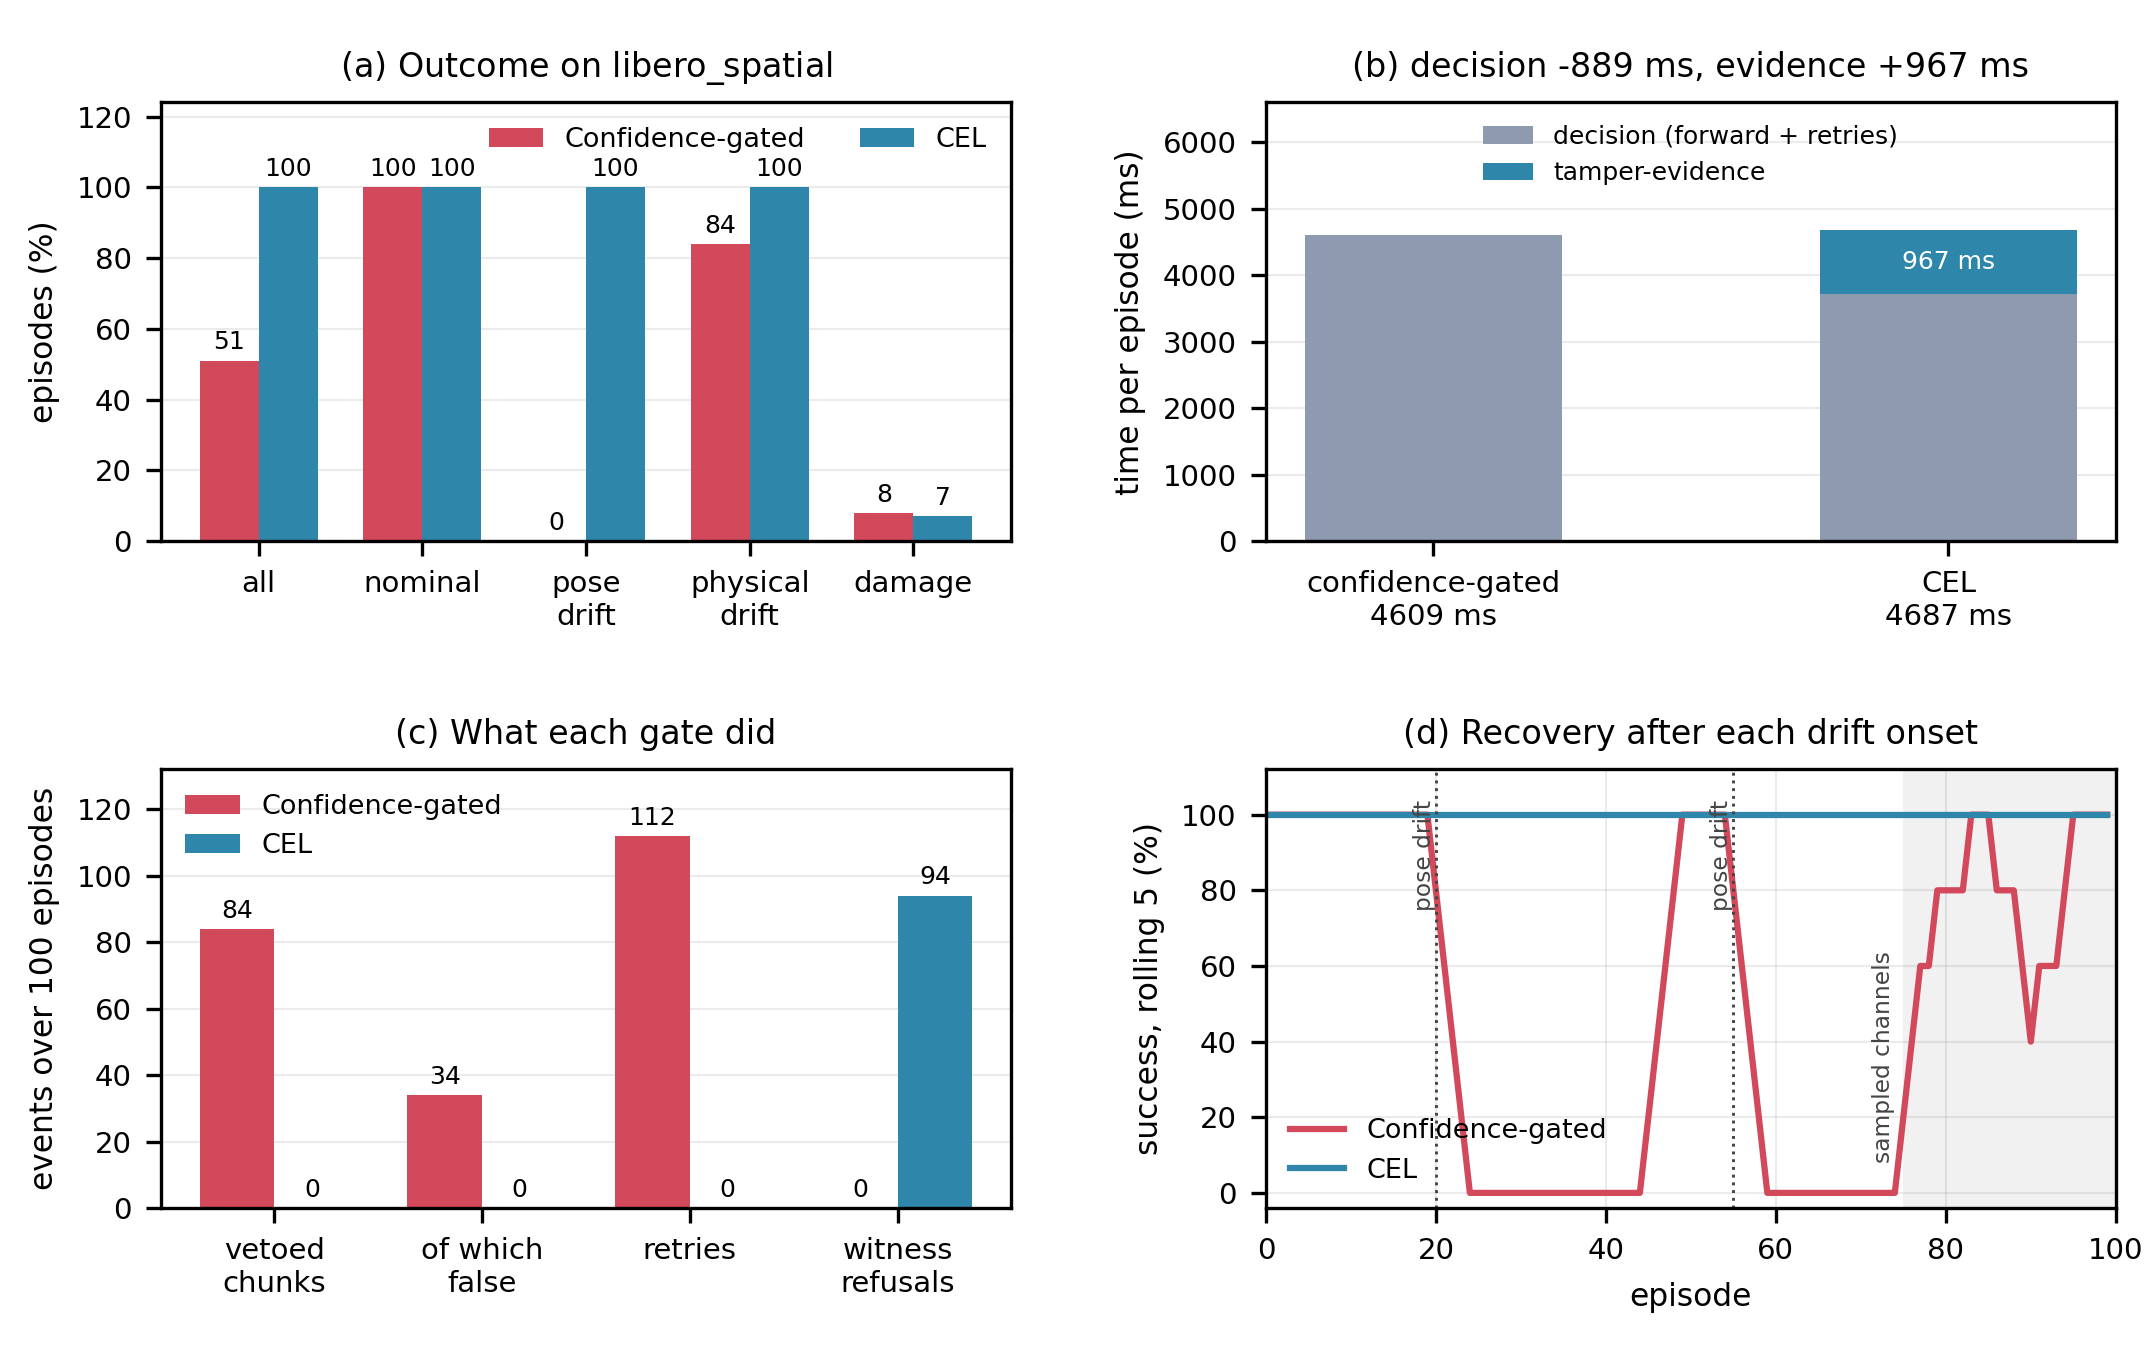
\includegraphics[width=\textwidth]{figures/libero_audit.png}
\caption{The manipulation audit, all four panels drawn from the run's own
episode records. (a) Outcome rates on \lib: overall success, success in the
nominal and pose-drift regimes, success over the drift channels, and the damage
rate. (b) Time per episode, split into the decision (forward passes and retries)
and the tamper-evidence; the split is the point, not the total, and the axis
carries both parts so the total can be read off. (c) What each gate did over the
hundred episodes---the baseline's vetoes, how many of them were false, and the
retries they cost, against the layer's refusals. The baseline cannot refuse at
all, which is why its last bar is empty rather than small. (d) Success over a
rolling window of five episodes, against the two pose-drift onsets: the layer
recovers inside the onset episode, the baseline never does.}
\label{fig:results}
\end{figure*}

\subsection{Success}

Table~\ref{tab:main} is the headline, and Fig.~\ref{fig:results}(a) is the same
numbers as bars so that the shape of the result is visible before the intervals
are read. At nominal, both arms are perfect:
\SafeNominal\%\ and \CELNominal\%, over \SafeNominalN{} episodes each. That
equality is the control---if the layer cost accuracy on the easy world, nothing
below would be interpretable.

Under pose drift the arms separate completely. Arm~A scores
\SafePoseDrift\%\ [\SafePoseDriftLo, \SafePoseDriftHi] and arm~B
\CELPoseDrift\%\ [\CELPoseDriftLo, \CELPoseDriftHi] over $\SafePoseDriftN$
episodes, a difference of \PoseGap{} points (Fisher exact \PoseP).

The mechanism is banal once stated. The plan froze a placement target when it
first looked at the scene; the plate then moved \PoseDeltaMin--\PoseDeltaMax\,mm. Arm~A executes
its stale target faithfully and sets the bowl down on empty table, finishing
\SafePosePlateDist\,mm from the plate on average. Its confidence is not low:
by the time the placement chunks run, the scene looks normal, the policy's
input is unremarkable, and there is nothing for a head trained on nominal data
to notice. Arm~B sees the plate's displacement at the first transport chunk,
refuses, re-derives targets from the new pose, and finishes
\CELPosePlateDist\,mm from the plate.

Recovery tells the same story per onset, and Fig.~\ref{fig:results}(d) shows it
per episode rather than as two numbers. Measuring episodes until the rolling
three-episode success rate returns to $0.8$: arm~A recovers after
\SafeRecoveryFirst{} and \SafeRecoverySecond{} episodes; arm~B after
\CELRecoveryFirst{} and \CELRecoverySecond. A baseline that never notices the
world moved cannot recover from it; the two numbers are not a difference of
degree.

On the four physical channels arm~A scores \SafeChannel\%\ and arm~B
\CELChannel\%. The honest reading is that those channels are \emph{easier} than
a \SI{100}{mm} plate displacement---Table~\ref{tab:regime} shows why: a
$\MassScale$-fold payload and a $\FrictionSlip$ friction coefficient mostly survive a nominal
grasp (measured lift \LiftPayload\,mm and \LiftSlip\,mm against
\LiftNominal\,mm at nominal), and \emph{light} is inert for a policy that reads
privileged state. Only the weakened actuator changes the arm as such
(\LiftActuator\,mm, \LiftActuatorPct\%\ of nominal). We report them as channels,
not as headline, and Table~\ref{tab:regime} reports each separately rather than
pooling five phenomena into one average.

\subsection{The baseline refuses the wrong things}

Arm~A vetoed \SafeVetoes\ chunks over $\EpisodesPerArm$ episodes, and
\SafeFalseVetoes\ of those refusals---\SafeFalseVetoRate\%\ [\SafeFalseVetoLo,
\SafeFalseVetoHi]---would have advanced the task. That is the metric a
confidence gate is never scored on, and it is the one that decides whether the
mechanism is usable.

The distribution in Fig.~\ref{fig:results}(c) is what makes the case that the
threshold is not tunable.
\SafeVetoesLightDim\ of the \SafeVetoes{} vetoes occur in the six
\emph{light} episodes, \SafeFalseVetoesLightDim\ of them false: the frame got
dark, so the head got unsure, so the arm stopped doing something that would
have worked. A further \SafeFalseVetoesNominal{} false vetoes occur at
\emph{nominal}---where by construction nothing has changed. Lower the threshold
and the light episodes stop being vetoed, but so do the drift episodes, because
the signal is one scalar driven by the frame; there is no value of it that
separates ``the world moved'' from ``the lamp dimmed''.

The layer has the opposite profile. Its $\CELRefusals$ refusals are all
measured mismatches between a registered prediction and an observed state, and
\CELRefusalsPose{} of them occur under pose drift. Its false-refusal count is
zero by construction, not by luck: a refusal means the digest the model
committed to was not the digest the world produced. When it is wrong about the
world, it is wrong in the direction the ledger records.

\subsection{Latency: the layer is cheaper where it decides}
\label{sec:latency}

Total latency per episode is \SafeLatency\,ms for arm~A and \CELLatency\,ms for
arm~B (Fig.~\ref{fig:results}(b), which also shows how the total divides): the
layer costs \LatencyDelta\,ms, \LatencyDeltaPct\%\ more. Taken
alone, that number would be a fair reason to reject the layer, and we do not
hide it. But the total is the sum of two things that are not alike.

\emph{Decision} latency---forward passes, gate reads, retries, re-derivations,
the work the policy does to choose an action---is \SafeLatency\,ms for arm~A and
\CELDecisionLatency\,ms for arm~B. The layer is \DecisionSaving\,ms
cheaper, \DecisionSavingPct\%\ less, because it never pays for a blind retry:
arm~A spends \SafeRetries{} forward passes on retries that end by executing
anyway, while arm~B's \CELReplans{} re-derivations are the whole of its extra
work and every one of them is a response to a measured failure.
\emph{Tamper-evidence} latency---the cost of proving the ledger was not
rewritten---is \CELWitnessLatency\,ms per episode for arm~B and zero for arm~A
by construction. Equation~\eqref{eq:latency} shows the split exactly.

\paragraph{The tamper-evidence term is a defect of ours, and it is
super-linear in the useful sense.} Every grant re-verifies the entire hash
chain before it is issued, so the price of a witness grows with the length of
the ledger that witnesses it. Table~\ref{tab:witnesscost}: \ChainSmallMs\,ms at
\ChainSmallEntries{} entries, \ChainMidMs\,ms at \ChainMidEntries,
\ChainLargeMs\,ms at \ChainLargeEntries---a factor of \ChainGrowth. The witness
itself, canonicalisation plus SHA-256, is \WitnessHashUs\,\textmu s. Over the
run the per-chunk cost is \CELWitnessPerChunk\,ms on average, \CELWitnessFirstTen\,ms
over the first ten episodes and \CELWitnessLastTen\,ms over the last ten; the
growth is entirely the chain check.

This is an implementation defect with a known shape, not a property of the
interface: an incremental accumulator or a Merkle root anchored periodically
makes verification $O(\log L)$ or $O(1)$ per grant, at the cost of a weaker
guarantee between anchors. We state the price curve rather than the fix because
the curve is what a deployment has to budget, and because a paper that reports
only the flattering decomposition would be doing what arm~A does.

\subsection{Damage, and what the layer does not prevent}

Contacts fall from \SafeCollisions{} (arm~A) to \CELCollisions{} (arm~B):
\SafeContactsPerEpisode{} against \CELContactsPerEpisode{} per episode. Damage
episodes are \SafeDamageEpisodes{} versus \CELDamageEpisodes---nearly equal,
and the reason is reported rather than smoothed: both arms drop the bowl four
times (\SafeDrops{} and \CELDrops{}), because a slip that happens during a
committed chunk is a slip that has already happened when the witness sees it. A
post-hoc witness cannot un-drop an object. What it can do is refuse to continue
placing a bowl it is no longer holding, and that is the difference visible in
the worst case: the largest final bowl--plate gap is \SafeWorstPlateDist\,mm
for arm~A and \CELWorstPlateDist\,mm for arm~B. The layer bounds the
\emph{consequence} of a failure it does not prevent.

\section{Generalization to Autonomous Driving}
\label{sec:driving}

\subsection{A trajectory is the same commitment}

An end-to-end driving planner does not emit a delta pose; it emits a trajectory
and a confidence. UniAD \cite{hu2023uniad} plans through a learned scene
representation and VAD \cite{chen2023vad} vectorises the scene and samples
plans; both are scored on whether the ego vehicle completes a route without
contact, on the distribution they were trained on. The interface question is the
one Section~\ref{sec:layer} asks, and in driving the blind spot is sharper than
in manipulation. Whether a pedestrian \SI{30}{m} ahead can be avoided is decided
by the coefficient of friction of the road, and no camera observes it: a wet
surface differs from a dry one in reflectance, not in geometry, and the encoder
has seen both. The literature has attacked this from the planning side, with
conformal guarantees re-estimated online when the environment shifts
\cite{rahaman2026environments}, and from the audit side, by measuring which
scene elements a deployed planner's decision actually depends on
\cite{guo2026cadet}. Both are statements about the plan and its inputs. Neither
measures what the vehicle did. A confidence head is therefore entitled to be
confident on a road it cannot stop on. The failure is not that the model is
wrong about the picture; it is that the picture does not contain the quantity
the plan depends on.

\subsection{Plant, route, and the two arms}

The simulator is replaced by the smallest model that contains the physics the
gate is blind to. The ego vehicle is a kinematic bicycle with a friction circle:
braking is capped at $\mu g$ and curvature at $\mu g/v^{2}$, so a wet road costs
stopping distance quadratically and cornering speed only linearly. Actuators are
first-order lags, $\dot a=(a_{\mathrm{cmd}}-a)/\tau_a$ and
$\dot\kappa=(\kappa_{\mathrm{cmd}}-\kappa)/\tau_s$, which is what a worn rack
is. The route is \SI{\ADRouteM}{m} of urban road with a queue at a red light, a
curve, a lead vehicle that either brakes at \SI{\ADLeadDecel}{m/s^2} or turns
off, and a pedestrian who steps out from behind parked vans when the ego is
\ADPedNear--\ADPedFar\,m away. The planner rolls out the \emph{nominal} plant
\ADHorizonS\,s ahead at \ADPlannerHz\,Hz and reports a confidence. Drift is
applied to the plant and never to that belief, so the rollout becomes wrong
while the policy stays the one from the control condition.

Arm~A is the confidence gate: below \ADConfThreshold{} it commands a
\SI{\ADEbDecel}{m/s^2} stop, otherwise it executes its trajectory blind.
Arm~B is the layer of Section~\ref{sec:layer}, transposed. At \ADWitnessHz\,Hz
it registers the plan's next waypoint as a tuple $(x,y,v)$ on the plan's grid,
quantises the observed tuple in the same frame, and grants execution only while
the discrepancy stays inside \SI{\ADTolLon}{m} longitudinally,
\SI{\ADTolLat}{m} laterally and \SI{\ADTolSpeed}{m/s} in speed; before each
re-plan it also demands that the road remaining is at least the stopping
distance implied by the grip it has \emph{measured}. A refusal re-plans from the
observed state with a jerk-limited take-over (\SI{\ADJerkLimit}{m/s^3}) written
\emph{inside} the new plan. That last clause is the lesson of
Section~\ref{sec:err004} one layer down: a take-over blended outside the plan
contradicts the waypoints the plan has just registered, refuses itself, and
cascades into a refusal loop.

Four worlds on one declared schedule, \ADEpisodesPerArm{} episodes per arm,
identical for both arms: nominal; wet ($\mu=\ADMuWet$ against a believed
$\ADMuNominal$); worn actuation ($\tau_s=\ADTauSWorn$\,s and
$\tau_a=\ADTauAWorn$\,s against \ADTauSNominal{} and \ADTauANominal{}); and both
together. The hazard is either the lead vehicle or the pedestrian, alternating
within every channel, so a channel is not also a hazard.

% Generated by make_numbers.py -- do not edit.
\begin{table*}[t]
\centering
\footnotesize
\setlength{\tabcolsep}{6pt}
\caption{The driving audit: \ADEpisodesPerArm{} episodes per arm, one declared schedule, identical planner and route. \emph{Coll.} counts episodes ending in contact with the lead vehicle or the pedestrian; \emph{cross-track p90} is the 90th percentile of an episode's largest lateral deviation from the lane centre; \emph{centre line} counts episodes that put a wheel over it (half-width \ADLaneHalf\,m). The last two columns exist because the success column cannot see the failure they count: in the worn-steering channel every baseline episode \emph{arrives}, and \ADLagPaintSafe\%\ of them put a wheel over the centre line on the way. \emph{Conf.} is the confidence-gated baseline of Section~\ref{sec:protocol}.}
\label{tab:driving}
\begin{tabular}{lrrrrrrrrr}
\toprule
 & & \multicolumn{2}{c}{\textbf{Collisions}} & \multicolumn{2}{c}{\textbf{Success (\%)}} & \multicolumn{2}{c}{\textbf{Cross-track p90 (m)}} & \multicolumn{2}{c}{\textbf{Centre line (\%)}} \\
\cmidrule(lr){3-4}\cmidrule(lr){5-6}\cmidrule(lr){7-8}\cmidrule(lr){9-10}
\textbf{World} & $\boldsymbol{n}$ & \textbf{Conf.} & \textbf{CEL} & \textbf{Conf.} & \textbf{CEL} & \textbf{Conf.} & \textbf{CEL} & \textbf{Conf.} & \textbf{CEL} \\
\midrule
nominal & 34 & 0 & 0 & 100 & 100 & 0.17 & 0.17 & 0 & 0 \\
wet road ($\mu=\ADMuWet$) & 30 & 15 & 0 & 50 & 100 & 0.14 & 0.12 & 0 & 0 \\
worn steering ($\tau_s=\ADTauSWorn$\,s) & 26 & 0 & 0 & 100 & 100 & 2.75 & 0.67 & 96 & 0 \\
wet $+$ worn & 10 & 5 & 0 & 50 & 100 & 1.48 & 0.41 & 10 & 0 \\
\midrule
all & 100 & 20 & 0 & 80 & 100 & 2.43 & 0.66 & 26 & 0 \\
\bottomrule
\end{tabular}
\end{table*}


\begin{figure*}[t]
\centering
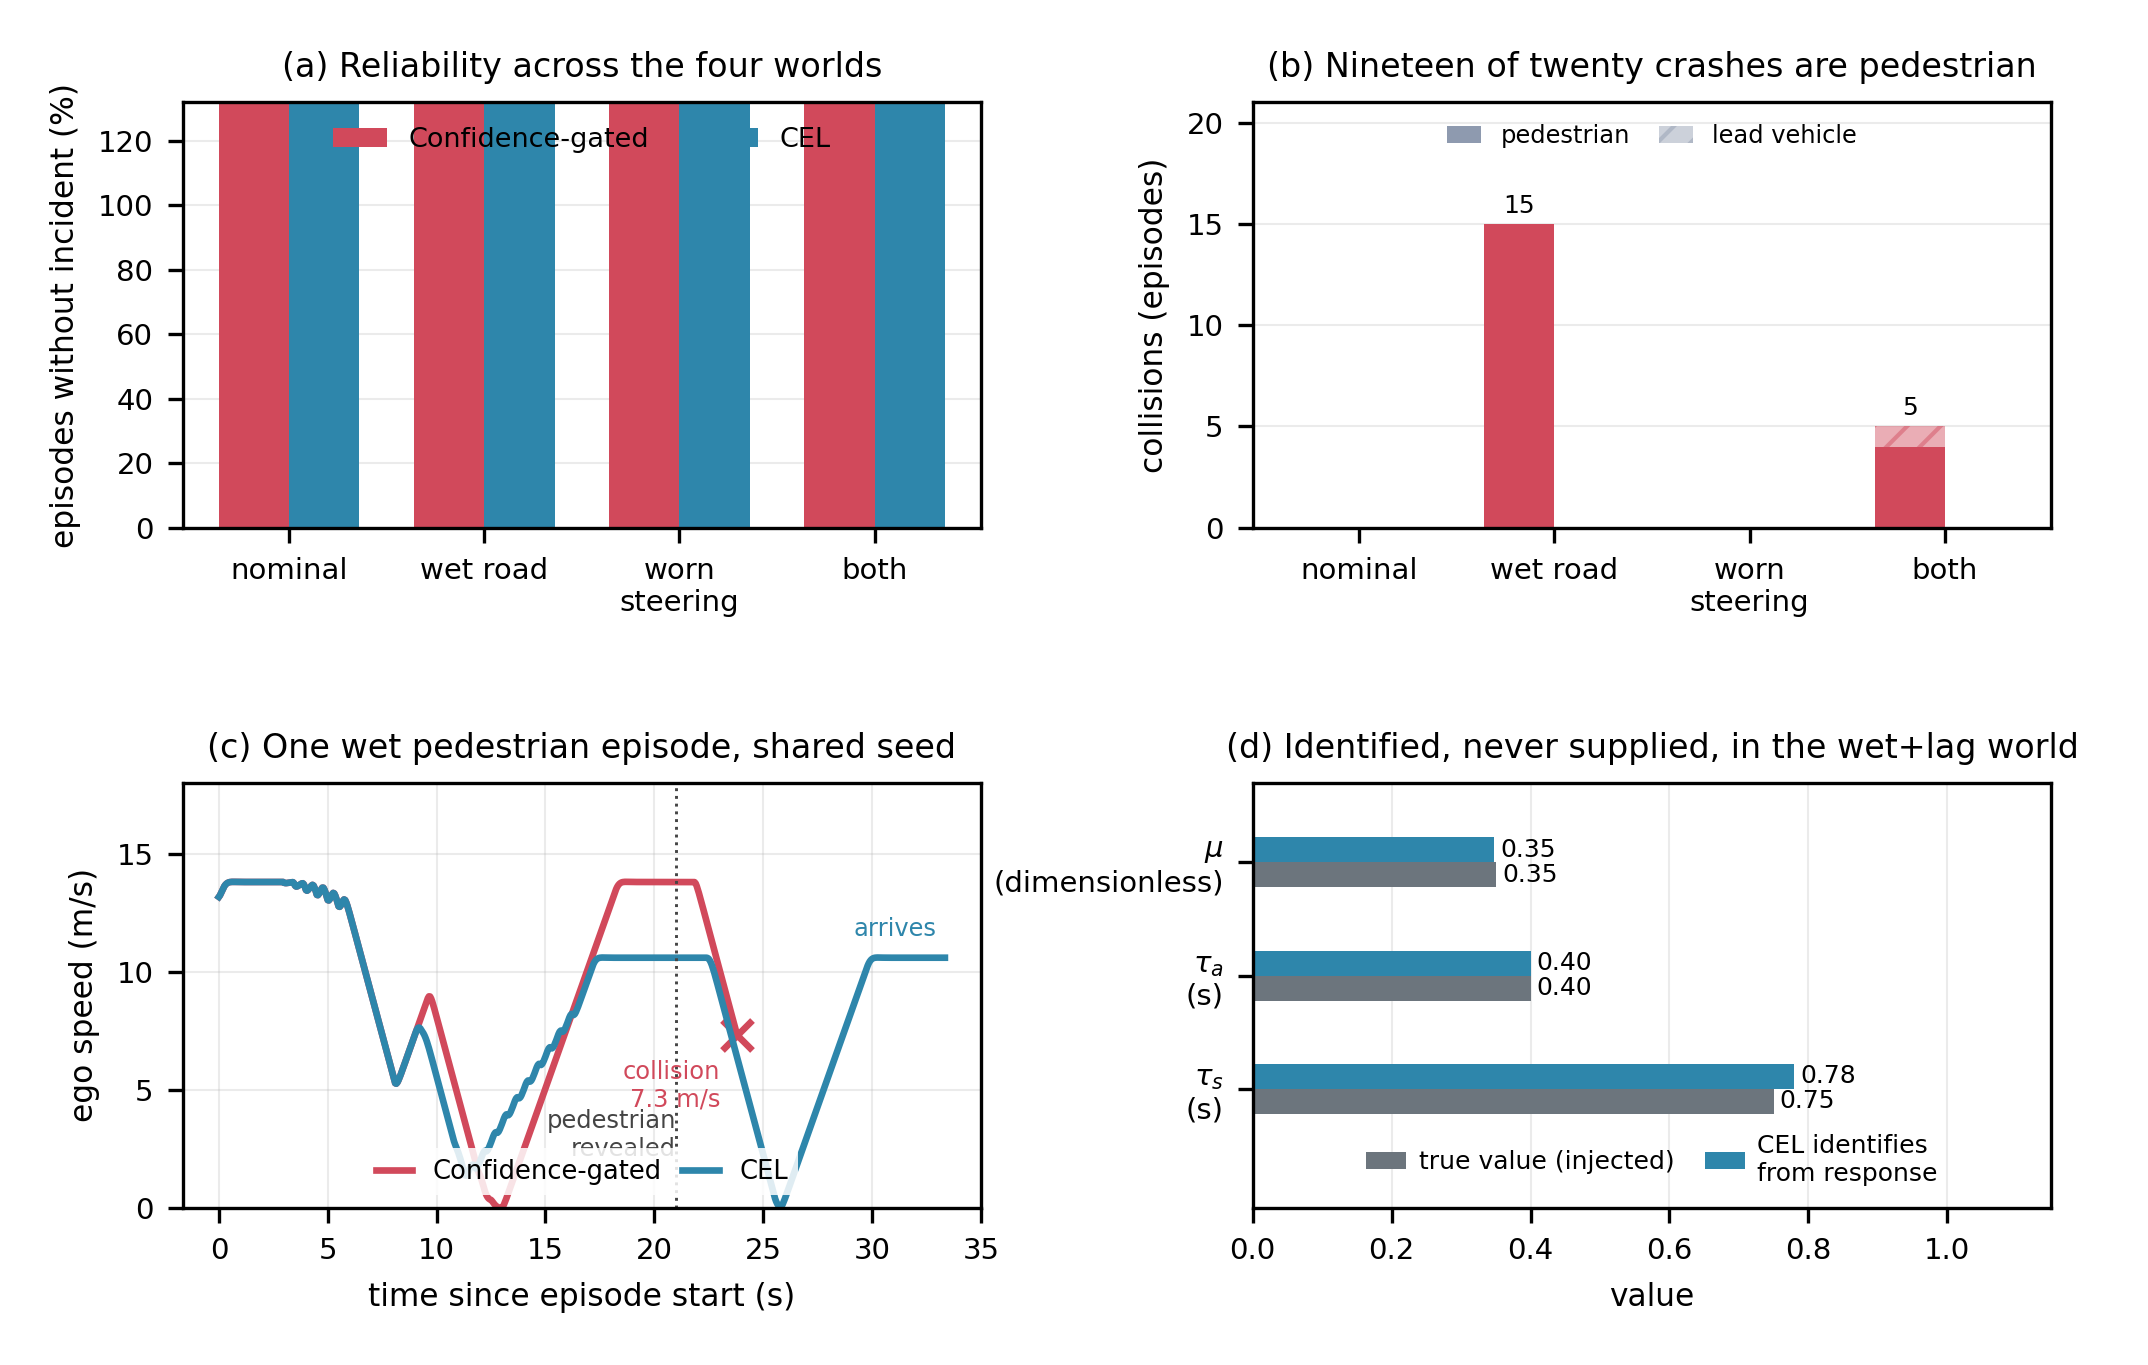
\includegraphics[width=0.94\textwidth]{figures/ad_cel.png}
\caption{The driving audit, drawn from the same records the tables are built
from. (a) Episodes without incident in each of the four declared worlds; the two
arms are indistinguishable in the nominal world and again under worn steering,
and they separate by half the episodes in the two wet worlds. (b) Collisions,
split by what was hit. Nineteen of the twenty are pedestrian; the single
lead-vehicle collision is in the wet-and-worn world. Every collision in both arms is
in a wet world: wetness is necessary, and the gate's confidence is not
sufficient. (c) One wet pedestrian episode, the same world and the same seed for
both arms (episode \ADTraceEp): ego speed against time, with the instant the
pedestrian becomes visible marked. At that instant the gate is at
\SI{\ADTraceVGate}{m/s} and the layer at \SI{\ADTraceVCEL}{m/s}, because the layer
had already priced the surface it measured. The layer's own braking command comes
later---\SI{\ADTraceGateBrakeDelay}{s} after the reveal for the gate,
\SI{\ADTraceCELBrakeDelay}{s} for the layer---but it starts from a speed that a
friction-limited stop can retire: it comes to rest \SI{\ADTraceCELStopT}{s} after the reveal and then
completes the route, while the gate is still doing \SI{\ADTraceImpact}{m/s} where
the pedestrian is. This is the section's whole argument in one trace: the
difference is not reaction time, it is the speed the reaction starts from.
(d) What the layer identifies in the wet-and-worn
world, against the values injected: grip from saturation, the two lags from the
step response. The baseline has no estimator and reports its prior in every
world ($\hat\mu=0.90$, $\hat\tau_a=0.10$\,s, $\hat\tau_s=0.08$\,s), which is the
blindness the figure is about.}
\label{fig:driving}
\end{figure*}

\subsection{Where the two are indistinguishable, and where they are not}

In the nominal world the two arms are the same instrument
(Fig.~\ref{fig:driving}(a), first pair of bars): zero collisions,
\ADNominalSuccSafe\%\ and \ADNominalSuccCEL\%\ arrivals, and
\SI{\ADNominalLatSafe}{m} of cross-track error for both. That equality is the
control; if the layer cost accuracy on the easy world, nothing below would be
interpretable.

On the wet road the gate loses half its episodes
(Fig.~\ref{fig:driving}(a)): success \ADWetSuccSafe\%\ against
\ADWetSuccCEL\%, i.e.\ \ADWetCollSafe{} collisions in \ADWetN{} against
\ADWetCollCEL{} for the layer (Fisher \ADWetCollP), with every one of those
crashes a pedestrian at \SI{\ADWetImpact}{m/s} mean impact speed and the mean gap
to the lead falling from \SI{\ADWetGapCEL}{m} to \SI{\ADWetGapSafe}{m}. Panel~(b)
is the same count split by what was hit. The mechanism is
arithmetic, and the audit computes it rather than asserting it. At the instant
the pedestrian becomes visible, a friction-limited stop fits inside the road
available with \SI{\ADWetDefSpare}{m} to spare on average, and the per-episode
deficit ranges from \ADWetDefMin{} (room to stop) to $+\ADWetDefMax$\,m
(already short). That average margin is smaller than the distance the car covers
while its planner reacts: the tracker's own \SI{\ADTrackLag}{s} time constant
is worth \SI{\ADWetLatDist}{m} at the \SI{\ADWetPedSpeed}{m/s} it was doing,
and the largest margin anywhere in the channel is \SI{\ADWetDefBest}{m}, so
the latency alone eats it in every one of the \ADWetCollSafe{} episodes even
where a friction-limited stop is calculated to fit. On dry tarmac
the same measurement leaves \SI{\ADNominalDefSpare}{m}, several times the
distance the latency costs. Wet tyres and worn actuators put the instant itself
at $+\SI{\ADWetLagDefSafe}{m}$: short before anything has moved.
Panel~(c) is that arithmetic in a single episode, the same seed for both arms:
the gate is at \SI{\ADTraceVGate}{m/s} when the pedestrian appears and is still
at \SI{\ADTraceImpact}{m/s} where she is.

The gate is not simply asleep. In \ADWetPedNoEB{} of the \ADWetPedN{} wet
pedestrian episodes it never fires, because nothing in the frame is wrong; in
the remaining \ADWetPedEB{} it fires and the car collides anyway, because a
\SI{\ADEbDecel}{m/s^2} command on a \ADMuWet{} road saturates at
$\mu g=\SI{\ADMuWetG}{m/s^2}$. The hardest stop the gate can ask for is a policy
constant, while the deceleration actually required is a property of the surface,
and the gate owns no measurement of the surface to compare its constant against.
This is the structural point in its purest form: the deficit is not a threshold
that was set too high, it is a quantity that is not in the input.

\subsection{The failure a success rate cannot see}

The worn-steering channel is the sharper result because every episode succeeds.
Both arms arrive in all \ADLagN{} episodes. The baseline's cross-track error at
the 90th percentile is \SI{\ADLagLatSafe}{m}, more than the \SI{\ADLaneHalf}{m}
half-width of the lane, and \ADLagPaintSafe\%\ of its episodes put a wheel over
the centre line, against \ADLagPaintCEL\%\ for the layer (Fisher
\ADLagPaintP). A plan tracked through a lagging rack oscillates across the lane
and still reaches the goal, so a benchmark that scores arrival rewards it.

The layer's \SI{\ADLagLatCEL}{m} comes from a predictor rather than a stiffer
gain. Having measured $\tau_s$, it aims the pursuit from the state the car will
be in $\hat\tau_s$ seconds from now, which cancels a pure delay that no feedback
gain can cancel without buying the oscillation it is trying to remove.

\subsection{Identification without privileged state}

Nothing in arm~B reads $\mu$, $\tau_a$ or $\tau_s$; all three are recovered from
the vehicle's own response. Grip comes from saturation: when the commanded
deceleration has been flat for twelve control steps and the realised value is
both large and below the command, the realised value \emph{is} the friction
limit, so $\hat\mu=|a|/g$. Lag comes from the step response, by inverting the
first-order solution over the same window. Medians over the run, and
Fig.~\ref{fig:driving}(d) puts them beside the injected values:
$\hat\mu=\ADMuHat$ against \ADMuWet{} true, $\hat\tau_a=\ADTauAHat$ against
\ADTauAWorn, $\hat\tau_s=\ADTauSHat$ against \ADTauSWorn{} (range
\ADTauSHatLo--\ADTauSHatHi), and $\hat\mu=\ADMuNominalHat$ on the dry episodes.
The layer then re-plans with the identified parameters, which is why its
stopping-distance witness is a statement about this road rather than about a
nominal one.

The estimator has a failure mode we hit and fixed. A first-order lag also makes
$|a|<|a_{\mathrm{cmd}}|$ for a few steps, so a braking transient looks exactly
like saturation; the first version therefore reported a wet road on dry tarmac
whenever it braked hard. Requiring a steady-state window before a deficit counts
as saturation removed it, and \texttt{tests/test\_ad\_cel\_audit.py} pins the
property on six nominal episodes.

\subsection{What the layer costs}

A confidence gate spends comfort to buy time; the layer spends time to buy
comfort. Over \ADEpisodesPerArm{} episodes per
arm the baseline spends \ADSafeHarsh{} hard-braked events against \ADCELHarsh{}
for the layer, of which \ADSafeEBN{} are emergency stops, and
\ADSafeEBFalseEp{} of its episodes are ones where the gate braked and the blind
replay arrives safely---refusals of a picture rather than of a world. The layer
refuses \ADCELRef{} times over \ADCELWitnessChecks{} witness checks;
\ADCELRefEp{} episodes carry at least one refusal, and every refusal is a
jerk-limited ramp inside the next plan rather than a \SI{\ADEbDecel}{m/s^2}
step, so the lurch a passenger would feel is the one arm~A makes.

Time is where the layer pays. Episode wall-clock rises from
\SI{\ADTimeEpSafe}{s} to \SI{\ADTimeEpCEL}{s}, $+\SI{\ADTimeEpDelta}{s}$ or
+\ADTimeEpPct\%, and that figure is not entirely honest:
\SI{\ADTimeEarlySafe}{s} of the baseline's mean is its twenty crashed episodes
ending early. Matched on episodes that reach the goal, the cost is
$+\SI{\ADTimeArrDelta}{s}$ (+\ADTimeArrPct\%), and in the nominal world, where
both arms arrive every time, the layer is \SI{\ADNominalTimeDelta}{s}
\emph{faster} (\ADNominalTimeSafe{} against \ADNominalTimeCEL{}\,s) because it
never brakes for a shadow. We report the flattering number and the corrected one
together, since the flattering one is the one that would be quoted.

\paragraph{What this does not show.} The plant is kinematic: no tyre model, no
load transfer, no perception, and the confidence is the same declared stand-in
used above, a scalar function of the frame with noise and a novelty penalty
rather than a trained head. One route geometry with one seeded hazard per
episode means the rates estimate a mechanism, not a fleet. $\mu=\ADMuWet$ and
$\tau_s=\ADTauSWorn$\,s are fault injections, not measured tyres: a wet road is
\ADMuWet, and a rack that lags \ADTauSWorn\,s is a failing one. The magnitudes
were chosen to be survivable by the layer and lethal to the gate; the ordering
is the claim. Finally, the driving ledger is a real chain: \ADRegistrations{}
registrations, \ADGrants{} grants and \ADLedgerRefusals{} refusals, re-walked
from its genesis hash and verified, with no replay offered and none accepted, so
the ordinal of Section~\ref{sec:err004} holds at \ADWitnessHz\,Hz for
\ADTotalEpisodes{} episodes.

\section{The Witness Must Be Bound in Time}
\label{sec:err004}

We now describe a defect in the layer we built, because it is the sharpest
evidence for the paper's thesis and because the first version of this
experiment produced a number that was wrong in the flattering direction.

\subsection{What the first run reported}

The first full run reported a success rate of $96.0\%$ for the layer, with
\textbf{zero} witness refusals in three episodes whose bowl finished
\SIrange{245}{269}{mm} from the plate.\footnote{Quoted from the pre-fix run's
console output. That run is not archived as a result: a run whose gate cannot
say no is preserved as a defect record, not as a table.} Every witness check in
those episodes was granted, the ledger verified, and the chain was intact.

\subsection{The mechanism: a replay}

Fig.~\ref{fig:replay} is the sequence below, drawn: registration adds to the
acceptable set, membership is never consumed, and a return to an earlier pose is
therefore indistinguishable from a fresh success.

The gateway keeps one set of acceptable digests per capability, and
registration adds to that set; an execution warranty is issued if the offered digest is a
member, and membership is never consumed. Canonicalising the scene alone
therefore made every chunk comparable with every earlier chunk of the same
episode. When the bowl slipped out of the gripper during transport and fell
back to the table, the observed canonical form was byte-identical to the form
registered ten chunks earlier, for the \textsf{close} stage, when the bowl
really was on the table:

\begin{center}
\small\ttfamily
\begin{tabular}{@{}ll@{}}
registered, chunk 3 & \texttt{scene@8,22,90:table}\\
expected,   chunk 10 & \texttt{scene@8,22,90:gripped}\\
observed,   chunk 10 & \texttt{scene@8,22,90:table}\\
\end{tabular}
\end{center}

\noindent and the gate granted a claim of \textsf{gripped} against an
observation of \textsf{table}. This is a replay attack in the protocol sense:
a recorded message, re-presented, accepted as fresh. The bowl returning to a
previously seen pose is not an exotic event; it is what gravity does.

\begin{figure}[!htbp]
\centering
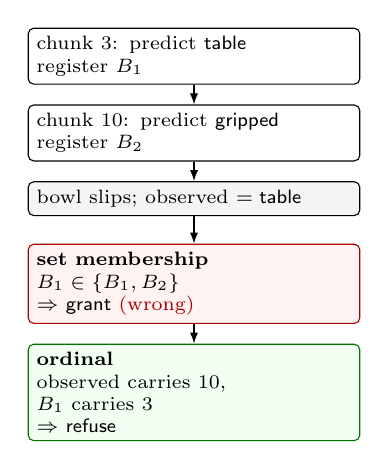
\begin{tikzpicture}[font=\scriptsize,
  n/.style={draw, rounded corners=2pt, align=left, inner sep=3pt,
            text width=40mm},
  bad/.style={n, draw=red!65!black, fill=red!5},
  good/.style={n, draw=green!45!black, fill=green!5},
  a/.style={-{Latex[length=1.4mm]}, semithick},
]
\node[n] (reg3) {chunk 3: predict \textsf{table}\\ register $B_1$};
\node[n, below=2.5mm of reg3] (reg10)
  {chunk 10: predict \textsf{gripped}\\ register $B_2$};
\node[n, below=2.5mm of reg10, fill=black!4] (slip)
  {bowl slips; observed $=\textsf{table}$};
\node[bad, below=3.5mm of slip] (set)
  {\textbf{set membership}\\
   $B_1\in\{B_1,B_2\}$\\
   $\Rightarrow$ \textsf{grant} \textcolor{red!65!black}{(wrong)}};
\node[good, below=2.5mm of set] (ord)
  {\textbf{ordinal}\\
   observed carries $10$,\\
   $B_1$ carries $3$\\
   $\Rightarrow$ \textsf{refuse}};
\draw[a] (reg3) -- (reg10);
\draw[a] (reg10) -- (slip);
\draw[a] (slip) -- (set);
\draw[a] (set) -- (ord);
\end{tikzpicture}
\caption{The replay, and the counter that closes it. The same scene at a
different attempt is a different event; a digest that binds only the scene
cannot tell them apart.}
\label{fig:replay}
\end{figure}

\subsection{Why hashing is not enough}

A hash is an equality test on \emph{content}. Causation is a relation between a
prediction and a \emph{particular attempt}, and two attempts may produce the same
content. Formally, $H(\kappa(s)) = H(\kappa(\hat{s}_{k+1}))$ is evidence that
$s$ equals $\hat{s}_{k+1}$; it is not evidence that $s$ is the consequence of
$a_k$. The gap is invisible whenever states are distinguishable, which is why it
survived development: the bowl on the table at the start and the bowl on the
table after a slip are the same bytes, and the interesting case is exactly the
one where they are.

This is the second instance of one failure in this line of work. In an earlier
system the witness omitted the difficulty of the gap it witnessed, so two
distinct claims shared one proof. Here the witness omits the identity of the
attempt, so two distinct events share one proof. In both cases the ledger
verifies, the chain passes, and the only symptom is a number that is too good.

\subsection{The fix: a one-shot ordinal}

Every registration is prefixed with a monotonically increasing ordinal, never
reset, and the check for that chunk carries the same ordinal:
\begin{equation}
\kappa'(s,k) = \texttt{chunk}_k \,\Vert\, \kappa(s).
\end{equation}
A registration is now redeemable exactly once, by the chunk that made it. A
regression cannot satisfy a stale prediction because no two predictions share a
key, and an episode boundary cannot alias an earlier episode's keys because the
counter lives on the gateway wrapper, not on the episode. The requirement
``registered before the request arrived'', which a set-membership gateway only
approximated, becomes a statement about the specific chunk.

The counter is a nonce, and the parallel is exact: authentication protocols have
used them for decades for the same reason. A physical witness needs one because
physical state is not injective in time---objects return to where they were.

\subsection{The corrected run, and what the defect cost}

After the fix, the same 200 episodes give \CELAll\%\ for the layer. The defect
had made the layer \emph{less} successful while making its ledger look
\emph{cleaner}: a false grant meant the plan continued to place a bowl it had
already dropped, so it failed at the end instead of refusing in the middle. Both
numbers are reported, and the pre-fix one is not archived as a result---it is
recorded here as a failure, which is the only honest place for it.

\section{Threats to Validity}
\label{sec:threats}

\paragraph{The policy is not a foundation model.} There is no OpenVLA checkpoint
in this environment, so the policy is a scripted chunked program and the
``forward pass'' is the declared constant $c_f$ of Section~\ref{sec:protocol}.
What that costs: the absolute latencies are a price list, not a measurement,
which is why Equation~\eqref{eq:latency} is printed. What it does not cost: the
comparison is between gates over an identical policy, and the policy is
open-loop within a chunk exactly as a VLA is. A better policy changes the
magnitudes, not the argument.

\paragraph{The confidence head is a model of a head.} Arm~A's confidence is a
scalar function of frame brightness with declared noise, not a trained head. A
better-calibrated head would veto less often, so our \SafeFalseVetoRate\%\ is a
property of this stand-in. But the argument is not calibration: a head consumes
the frame, and the frame does not contain the plate's displacement. The
\emph{light} channel is where this is least ambiguous, and there the head
behaves exactly as a well-calibrated head should---it notices the input changed
and refuses \SafeVetoesLightDim\ times, \SafeFalseVetoesLightDim\ of them
wrongly. Calibration moves that number; it does not move it to zero.

\paragraph{Privileged state.} The layer reads simulator ground truth. A real
deployment needs a state estimator, and the witness is only as good as that
estimator is accurate relative to the grid. We chose \GridMm\,mm, five times
the observed settling; a perception stack with, say, \SI{15}{mm} noise would
need a coarser grid and would be correspondingly less sensitive. The drift
audit measures the image channel separately for this reason and reports
\emph{light} as inert for this policy rather than as a capability difference.

\paragraph{One task, one seed, 100 episodes per arm.} The intervals in
Table~\ref{tab:main} are the honest statement of that limit. The pose-drift
result ($0/45$ against $45/45$, \PoseP) is far outside sampling noise; the
reported \CELAll\%\ should be read as ``above \CELAllLo\%'', not as a
measurement of a rate.

\paragraph{Injected drift is parametric.} Friction, mass, light, actuator gain
and a rigid displacement. Real drift includes geometry change, occlusion,
sensor failure and human interference. The layer's dependence on being able to
\emph{classify} the observed state is a genuine scope limit: under occlusion the
witness can be unable to answer, and the correct behaviour there is to refuse,
which we do not test.

\paragraph{Prior-art coverage is not exhaustive.} The scripted sweep of arXiv
and Semantic Scholar could not be completed: both agencies answered every keyword
query with HTTP~429 from this host throughout the audit, so the sweep returned no
records. It was replaced by a manual search of the same eight phrases over
2023--2026---\emph{causal execution layer}, \emph{safe VLA}, \emph{end-to-end
autonomous driving}, \emph{world model}, \emph{physical hallucination},
\emph{metabolic solidification}, \emph{safety filter} for VLA, and
\emph{runtime verification} for manipulation---with every candidate confirmed
against its arXiv abstract page. A manual sweep carries no recall guarantee: an
isomorphic work this vocabulary does not reach may exist, so the novelty claims
here are claims about the works cited, not about the literature.

\paragraph{The chain cost is measured on a local filesystem.} Table
\ref{tab:witnesscost} is a tmpfs measurement; on a network store, fsync
dominates and the constant is worse. The scaling, not the constant, is the
finding.

\section{Future Work}

\paragraph{Sub-linear tamper-evidence.} Incremental verification with a
periodically anchored Merkle root is the obvious fix for
Section~\ref{sec:latency}; the open question is what guarantee survives between
anchors and how much a deployment should pay for it. This is the one item on
this list that is a defect rather than an extension.

\paragraph{Sequences, not chunks.} An ordinal binds one attempt. A causal trace
should bind a \emph{partial order} of attempts, so that a plan can be refused
for the shape of its history and not only for the last step---for example when
three re-derivations in a row are evidence of a model that is wrong about the
mechanism, not unlucky.

\paragraph{Learned witnesses.} The classification used here is geometric and
hand-declared. A learned witness that maps proprioception and vision to the same
canonical form would remove the privileged-state assumption; the risk is the
obvious one, that the witness inherits the policy's blindness.

\paragraph{When is a witness worth its price?} The layer costs a measurable
per-chunk amount and returns success under drift. The ratio should be predicted
before it is measured: a witness is worth buying while its price is below the
drift rate times the cost of a failure, which is the same inequality that
governs a compiled rule in a metabolising system. Our \CELWitnessPerChunk\,ms
against a \SafeLatency\,ms episode is one point on that curve, not the curve.

\paragraph{Real foundation models, more tasks, more seeds.} The next experiment
is this protocol with an OpenVLA checkpoint and the LIBERO-90 suite, where the
relative cost changes because a real forward pass is expensive next to a witness.

\section{Conclusion}

A confidence gate and a physical witness answer different questions. The first
asks how sure the model is; the second asks whether the world did what the model
said. On a real LIBERO task, under a target that moves \SI{100}{mm} after the
plan is written, those questions get different answers: \SafePoseDrift\%\
against \CELPoseDrift\%, with the confidence baseline refusing
\SafeFalseVetoRate\%\ of the actions it vetoed and the layer refusing none that
would have worked. The layer's decision latency is lower than the baseline's,
because a blind retry is more expensive than a measurement; its total latency is
higher, because our ledger verification is linear in the ledger, which we report
as a defect.

The same question, asked of a vehicle instead of an arm, gets the same answer
under a drift no camera can see: on a wet road the gate ends \ADWetCollSafe{} of
\ADWetN{} episodes in a pedestrian collision and the layer ends none, and on a
worn steering rack both arms arrive while only the layer arrives in its own lane
(\ADLagPaintSafe\%\ against \ADLagPaintCEL\%\ over the centre line). The layer
recovers the friction and the lags from its own saturated and stepped responses,
so nothing in that comparison depends on privileged state. A witness that commits
to a physical consequence is portable across embodiments because it is a claim
about the world---the same world in both experiments, which is more than can be
said for a confidence.

The most useful result is the one that went wrong. Our first gate accepted a
scene that had returned to a state it had predicted earlier, because the gate
tested membership in a set of digests rather than identity of an attempt. A hash
binds content; causation binds a prediction to an attempt, and the difference
between those two is exactly the case where the world undoes your work. The
monotonic ordinal that closes it is one line. Finding that it was needed took a
run whose numbers looked good.

\section*{Reproducibility}

Every number in this paper is generated.
\code{experiments/benchmark\_libero\_audit.py} runs the
$\TotalEpisodes$ episodes and writes \code{libero\_audit\_episodes.csv},
\code{libero\_audit\_summary.json} and the hash-linked ledger;
\code{experiments/cel\_paper/make\_numbers.py} turns those into the
\code{data/*.tex} macros and tables this document inputs. The artifact was not
committed from the author's working tree; the commands and the pinned versions
(\code{mujoco==\MujocoVersion}, \code{robosuite==\RobosuiteVersion}) are in the
repository's \code{experiments/README.md}, and the defect of
Section~\ref{sec:err004} is \code{ERR-004} in its \code{ERRATA.md}.

\bibliographystyle{IEEEtran}
\bibliography{references}

\end{document}
